% !TEX root = ../main.tex

% 中英标题:\chapter{中文标题}[英文标题]
\chapter{排版图片}[Typesetting pictures]

\section{引言}[Introduction]
图应有自明性。插图应与文字紧密配合,文图相符,内容正确。选图要力求精练,插图、照
片应完整清晰。机械工程图:采用第一角投影法,严格按照GB4457~GB131-83《机械制图》
标准规定。数据流程图、程序流程图、系统流程图等按GB1526-89标准规定。电气图:图形
符号、文字符号等应符合附录3所列有关标准的规定。流程图:必须采用结构化程序并正确
运用流程框图。对无规定符号的图形应采用该行业的常用画法。坐标图的坐标线均用细实线
,粗细不得超过图中曲线;有数字标注的坐标图,必须注明坐标单位。照片图要求主题和主
要显示部分的轮廓鲜明,便于制版。如用放大或缩小的复制品,必须清晰,反差适中。照片
上应有表示目的物尺寸的标度。引用文献中的图时,除在正文文字中标注参考文献序号以外
,还必须在中、英文表题的右上角标注参考文献序号。

\section{博士毕业论文双语题注}[Doctoral picture example]

博士毕业论文双语题注如\figref{golfer1}所示。

\begin{figure}[htpb]
\centering
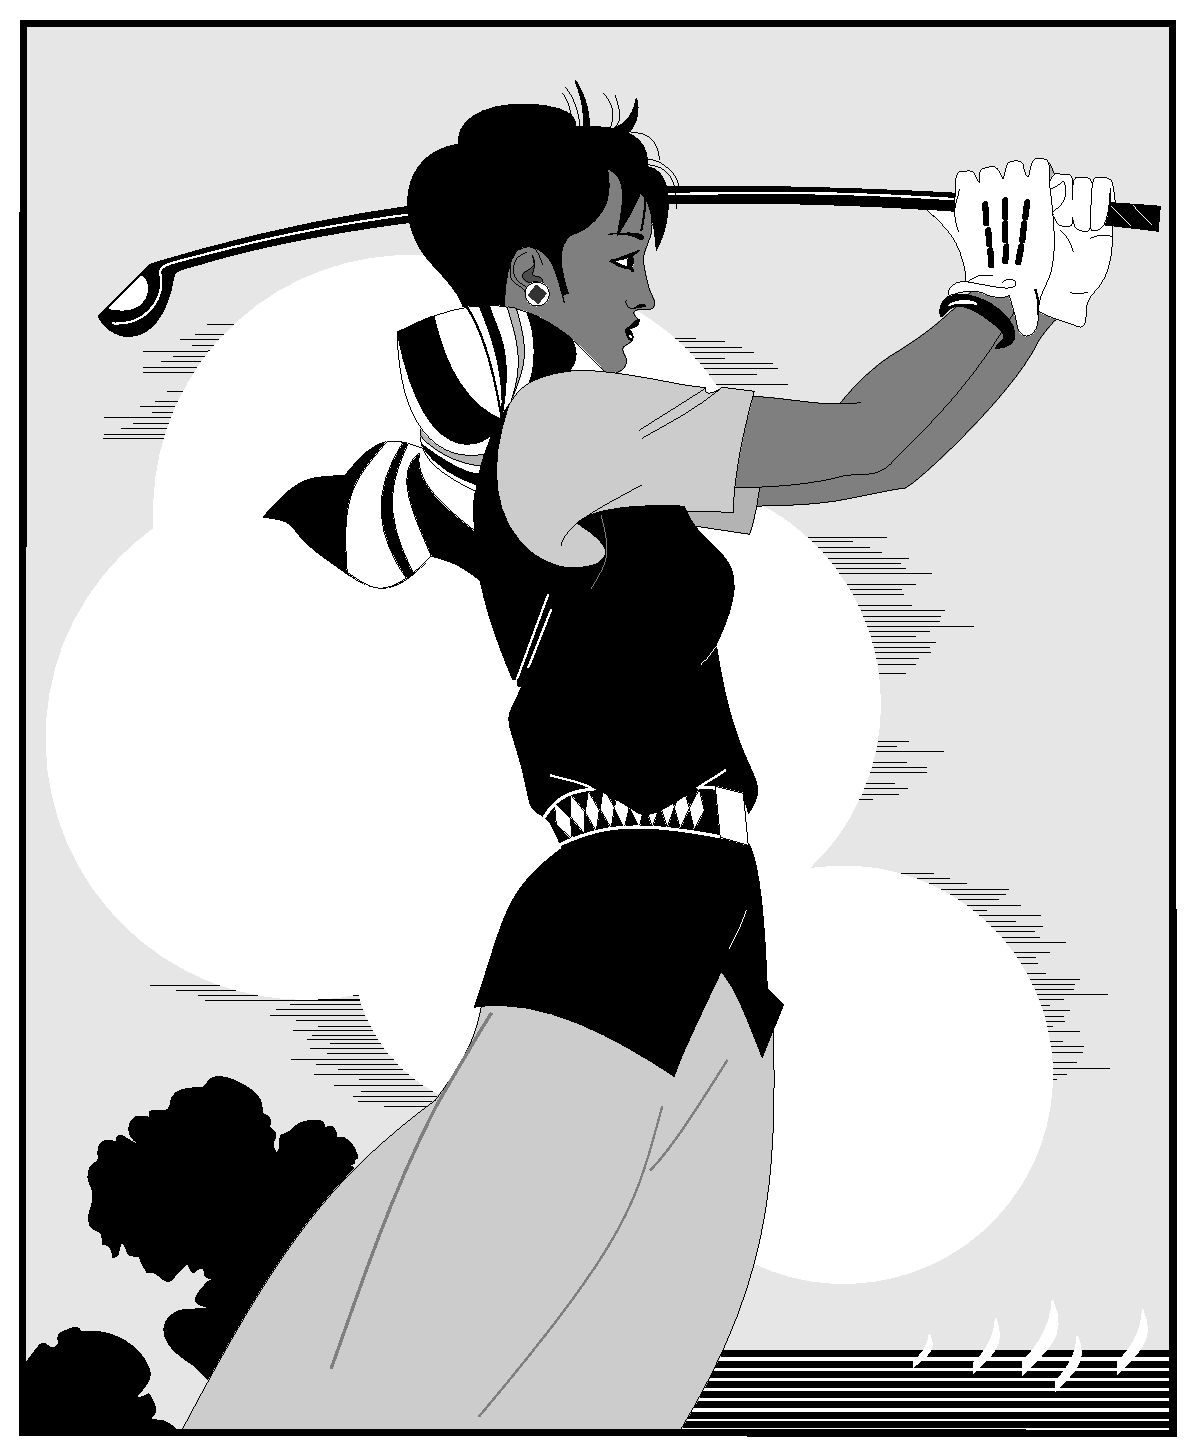
\includegraphics[width = 0.4\textwidth]{golfer}
\bicaption[golfer1]{}{打高尔夫球球的人(博士论文双语题注)}{Fig.$\!$}{The person playing golf (Doctoral thesis)}
\end{figure}

每个图均应有图题(由图序和图名组成),图题不宜有标点符号,图名在图序之后空1个半
角字符排写。图序按章编排,如第1章第一个插图的图号为“图1-1”。图题置于图下,硕士论
文只用中文,博士论文用中、英两种文字,居中书写,中文在上,要求中文用宋体5号字,
英文用Times New Roman 5号字。有图注或其它说明时应置于图题之上。引用图应注明出处
,在图题右上角加引用文献号。图中若有分图时,分图题置于分图之下或图题之下,可以只
用中文书写,分图号用a)、b)等表示。图中各部分说明应采用中文(引用的外文图除外)或
数字符号,各项文字说明置于图题之上(有分图时,置于分图题之上)。图中文字用宋体、
Times New Roman字体,字号尽量采用5号字(当字数较多时可用小5号字,以清晰表达为原
则,但在一个插图内字号要统一)。同一图内使用文字应统一。图表中物理量、符号用斜体
。
\subsection{本硕论文题注}[Other picture example]

本硕论文题注如\figref{fig:bm}所示。

\begin{figure}[ht]
\centering
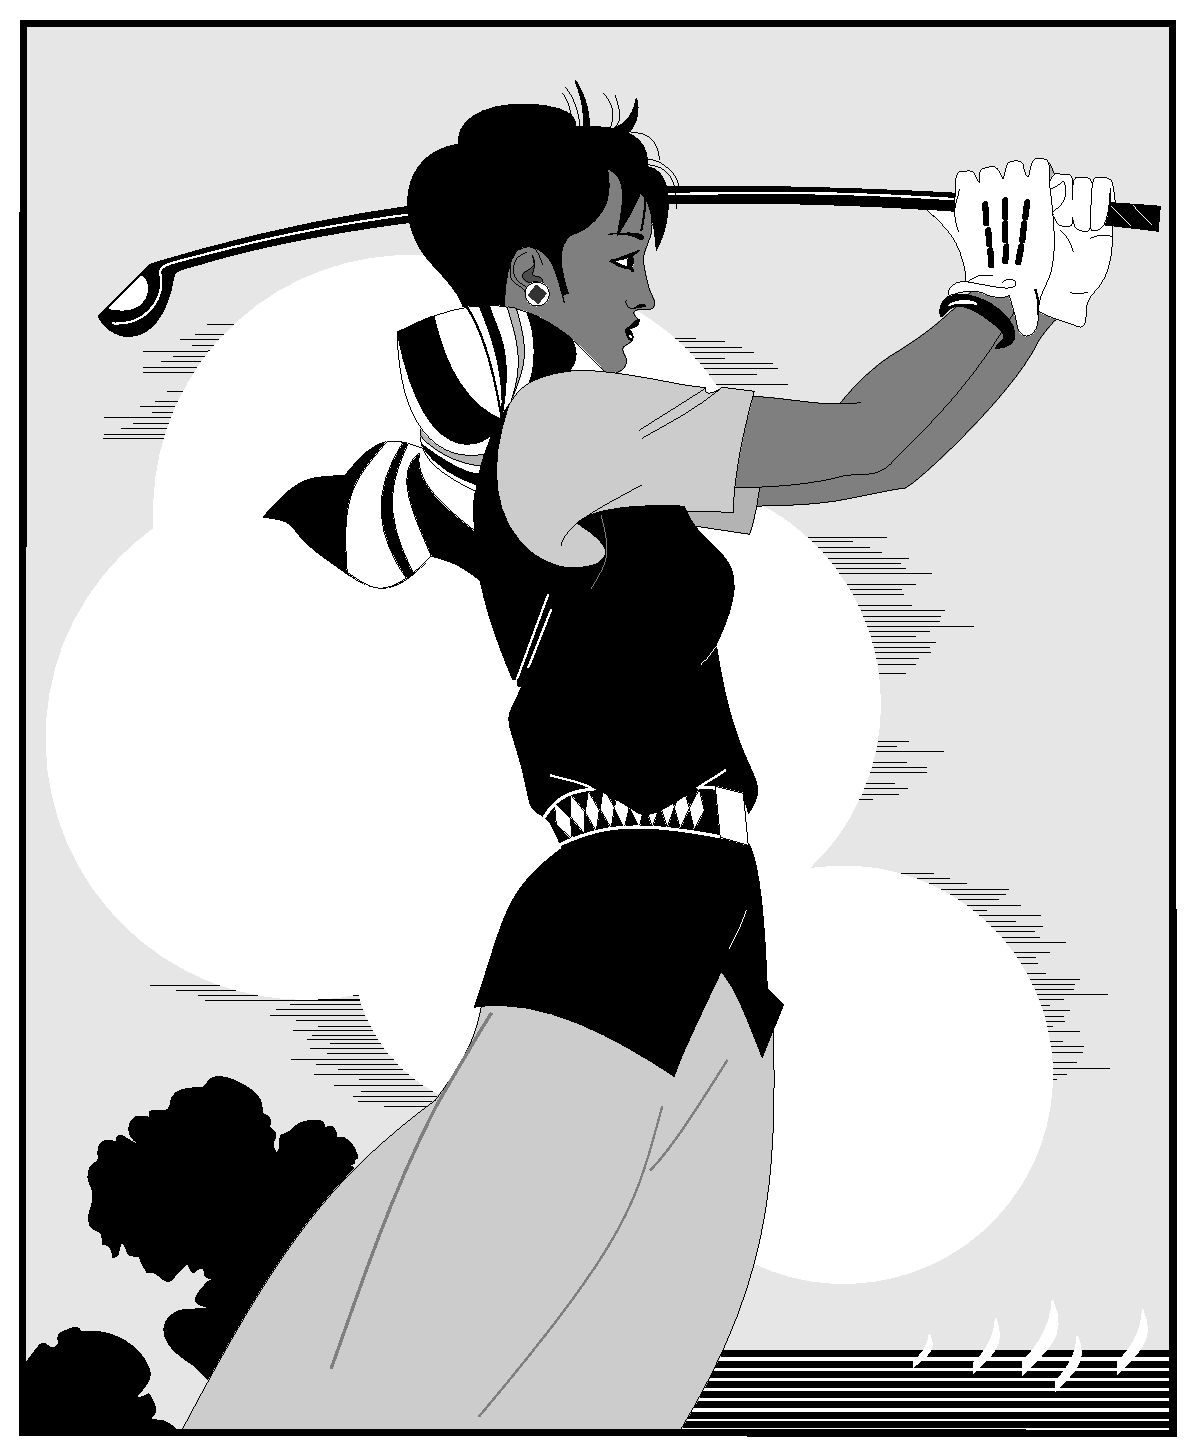
\includegraphics[width = 0.4\textwidth]{golfer}
\caption{打高尔夫球的人,硕士论文要求只用汉语}
\label{fig:bm}
\end{figure}

\subsection{并排图和子图}[Abreast-picture and Sub-picture example]
\subsubsection{并排图}[Abreast-picture example]

使用并排图时,需要注意对齐方式。默认情况是中部对齐。这里给出中部对齐、顶部对齐
、图片底部对齐三种常见方式。其中,底部对齐方式有一个很巧妙的方式,将长度比较小
的图放在左面即可。

\lipsum[2]

\begin{figure}[htbp]
\centering
\begin{minipage}{0.4\textwidth}
\centering
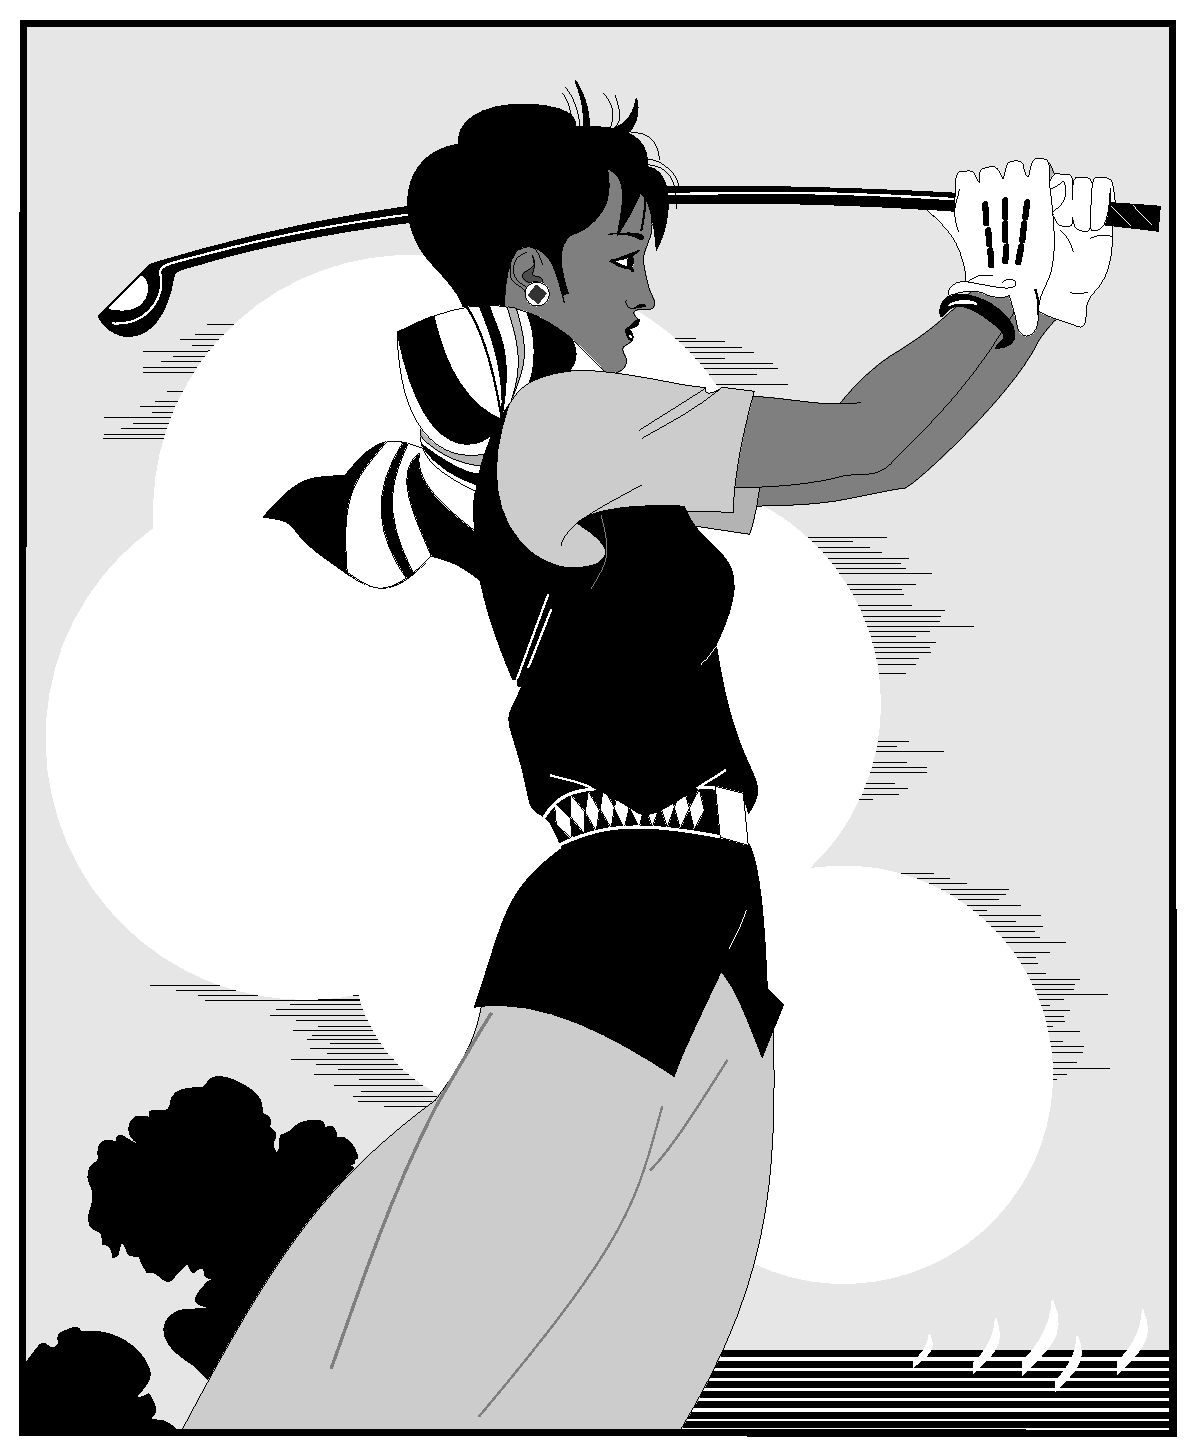
\includegraphics[width=\textwidth]{golfer}
\bicaption[golfer2]{}{打高尔夫球的人}{Fig.$\!$}{The person playing golf}
\end{minipage}
\centering
\begin{minipage}{0.4\textwidth}
\centering
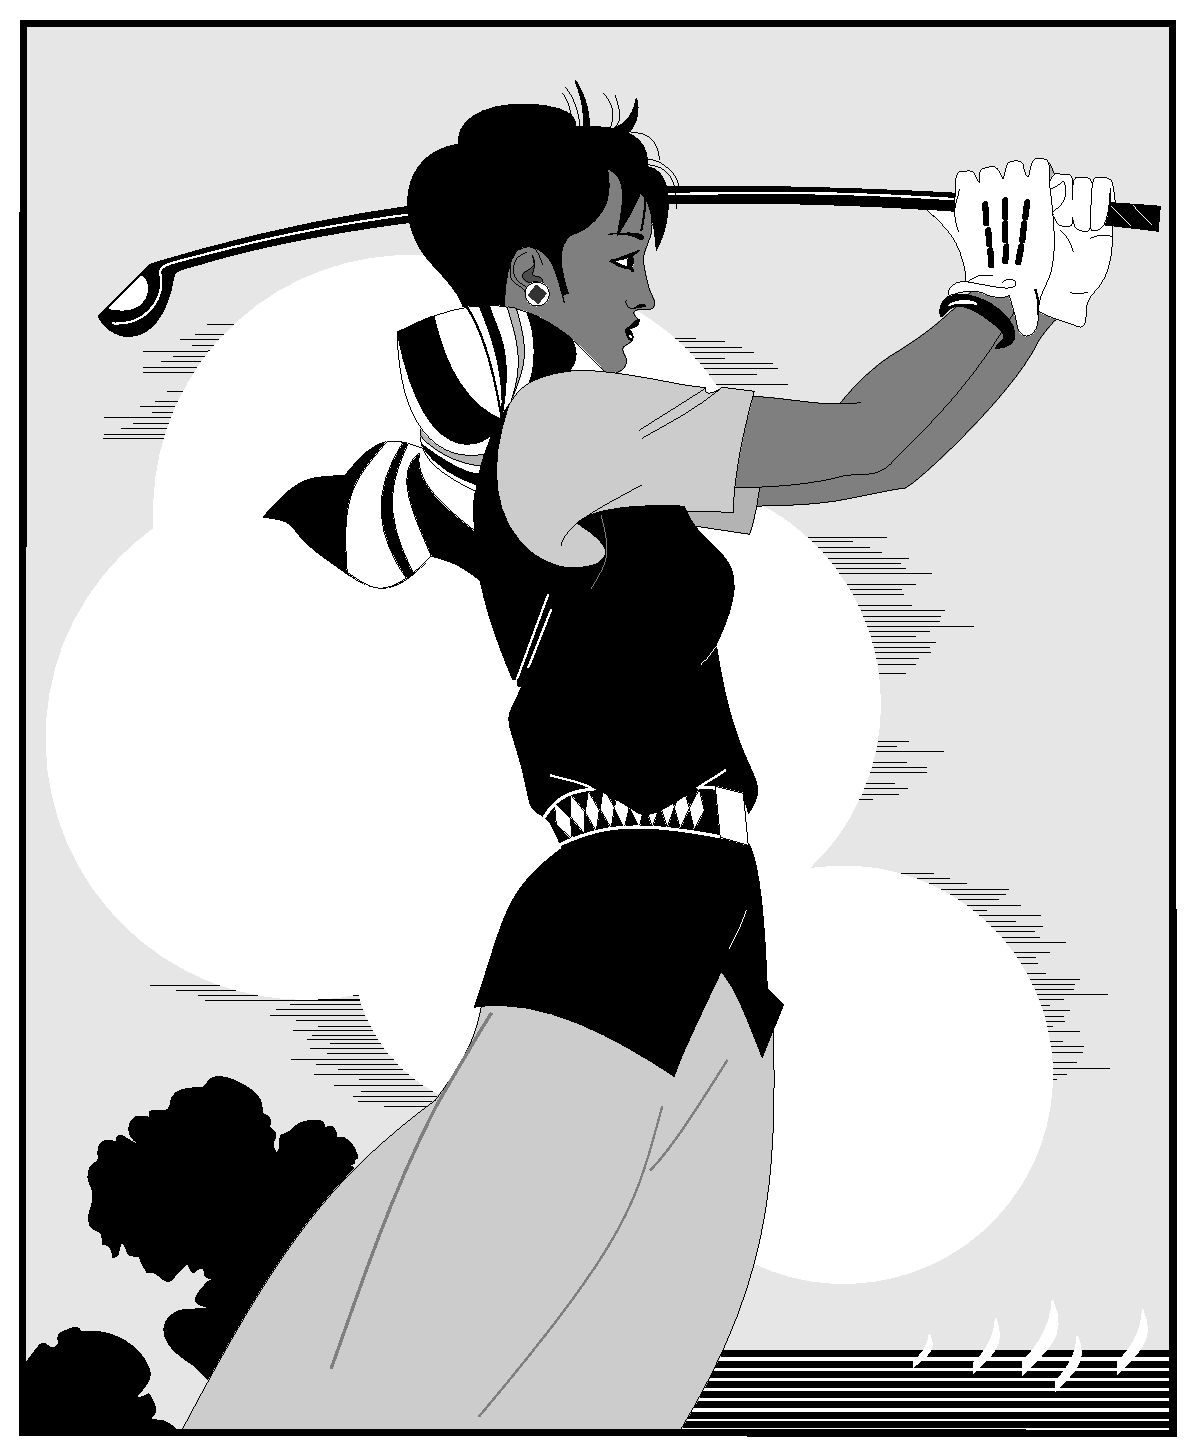
\includegraphics[width=\textwidth]{golfer}
\bicaption[golfer3]{}{打高尔夫球的人。注意,这里默认居中}{Fig.$\!$}{The person playing golf. Please note that, it is vertically center aligned by default.}
\end{minipage}
\end{figure}

\begin{figure}[htbp]
\centering
\begin{minipage}[t]{0.4\textwidth}
\centering
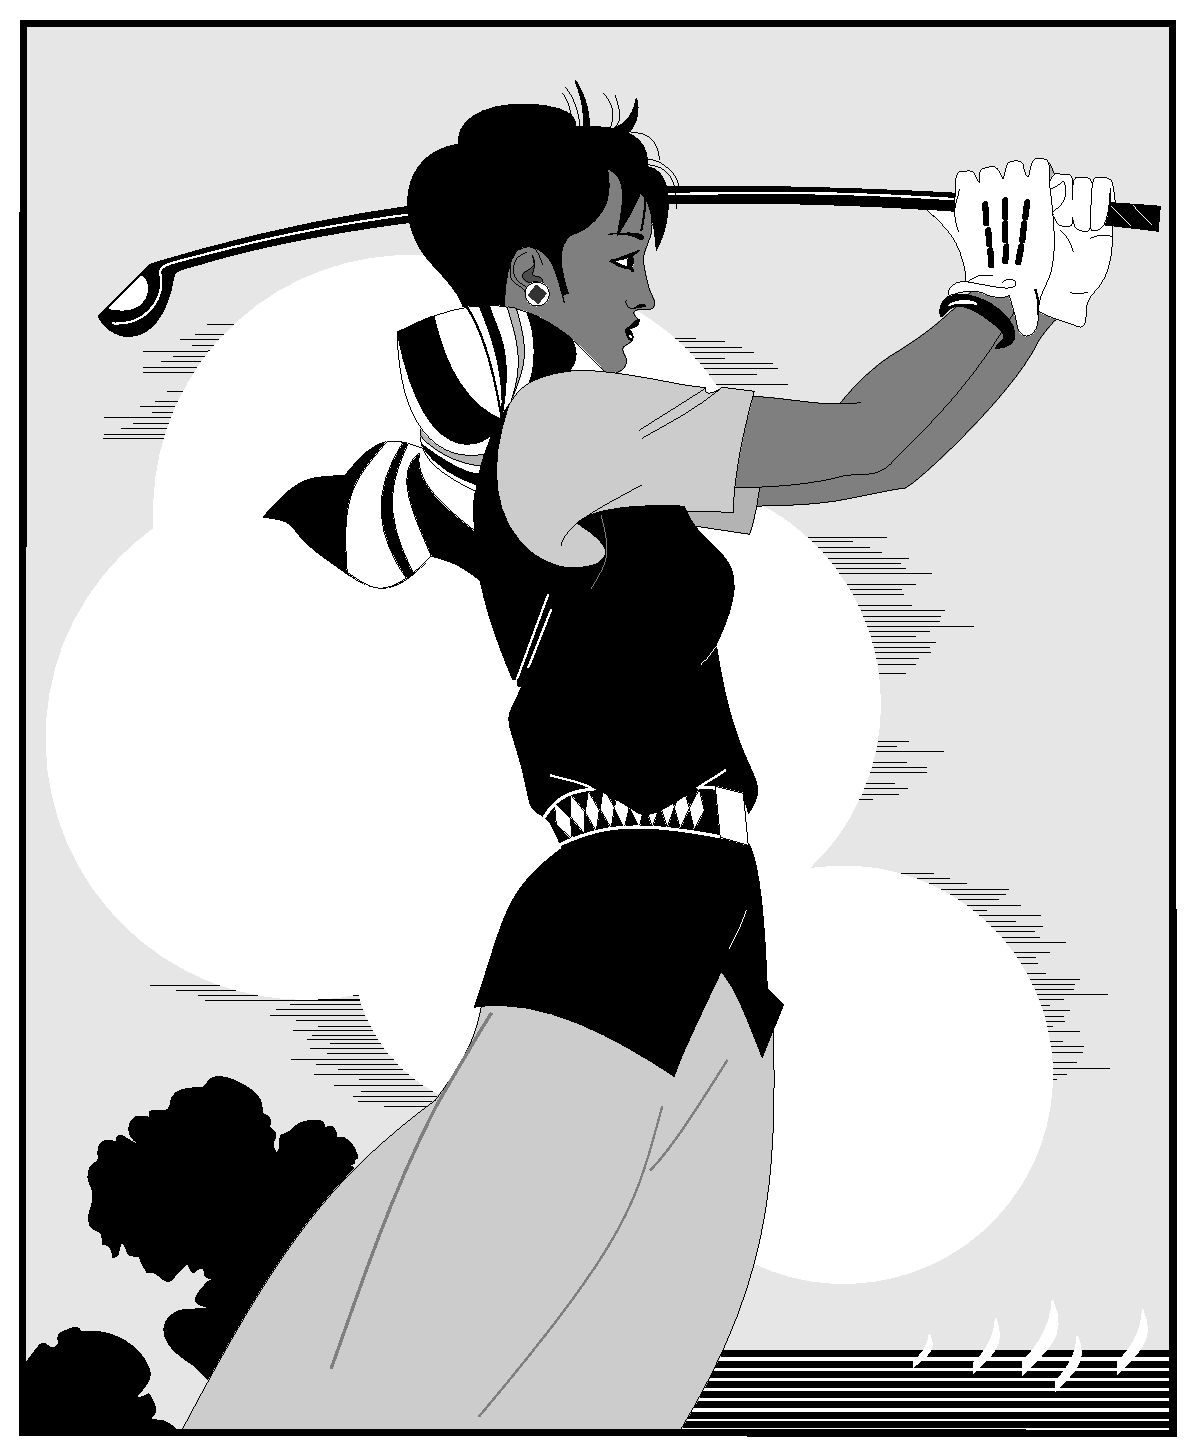
\includegraphics[width=\textwidth]{golfer}
\bicaption[golfer5]{}{打高尔夫球的人}{Fig.$\!$}{The person playing golf}
\end{minipage}
\centering
\begin{minipage}[t]{0.4\textwidth}
\centering
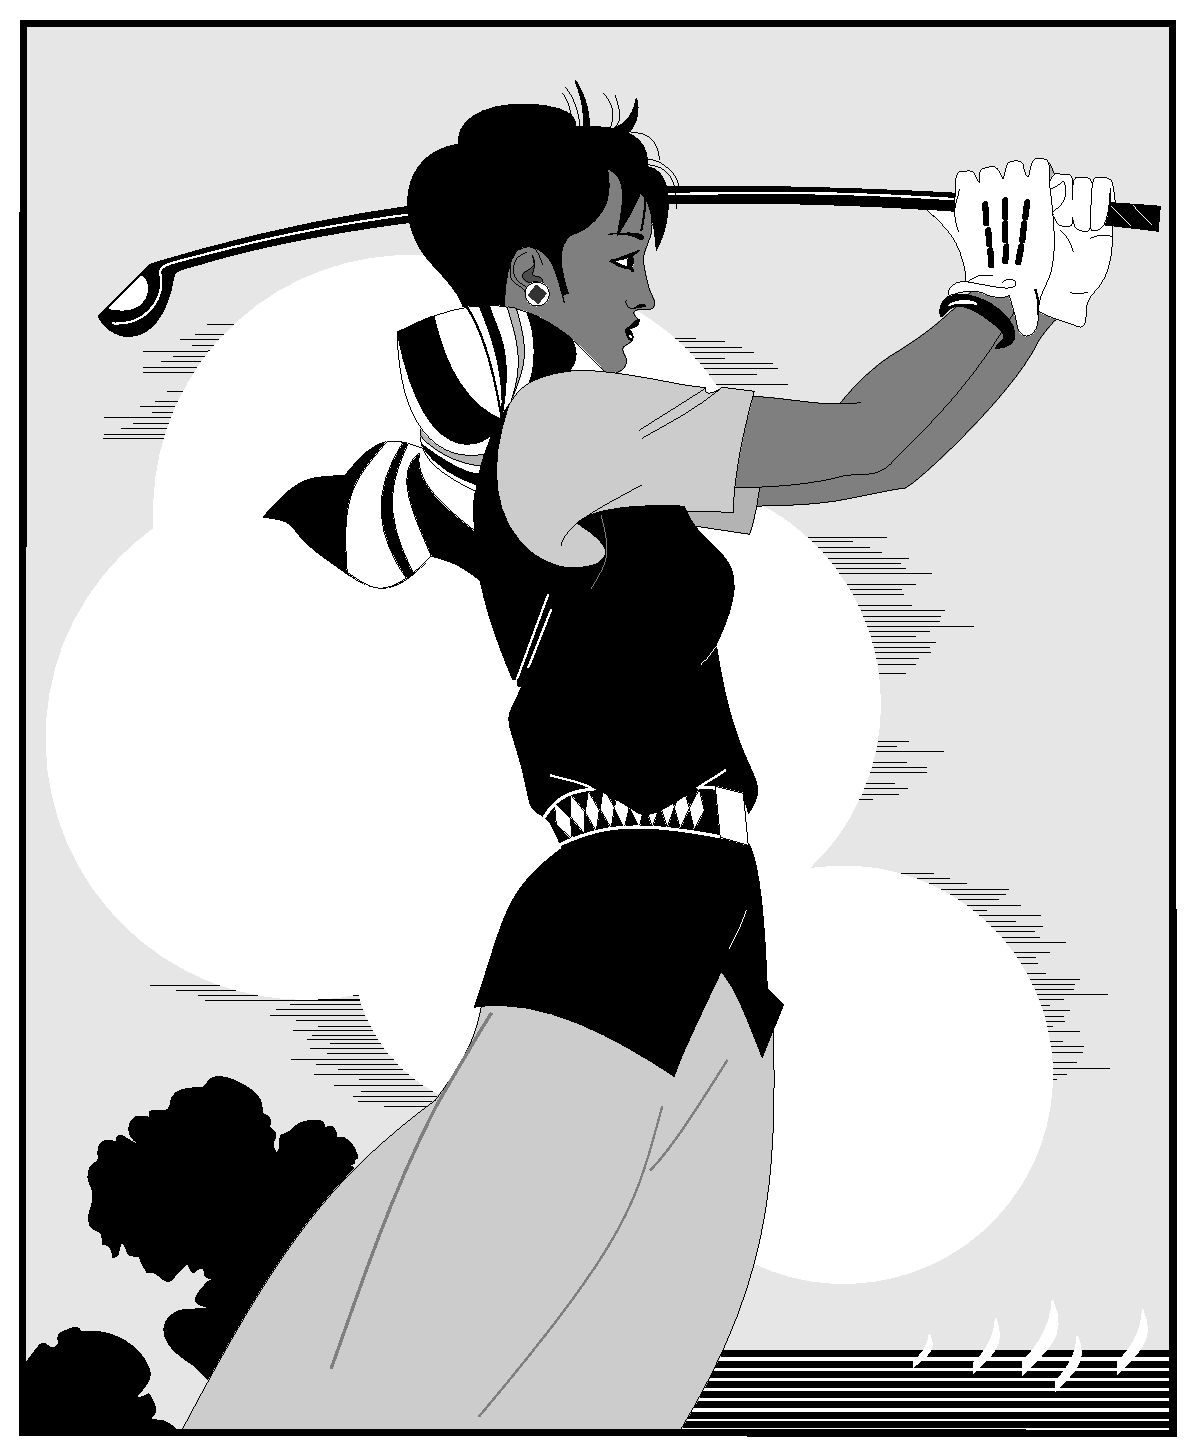
\includegraphics[width=\textwidth]{golfer}
\bicaption[golfer8]{}{打高尔夫球的人。注意,此图是顶部对齐}{Fig.$\!$}{The person playing golf. Please note that, it is vertically top aligned.}
\end{minipage}
\end{figure}

\begin{figure}[htbp]
\centering
\begin{minipage}[t]{0.4\textwidth}
\centering
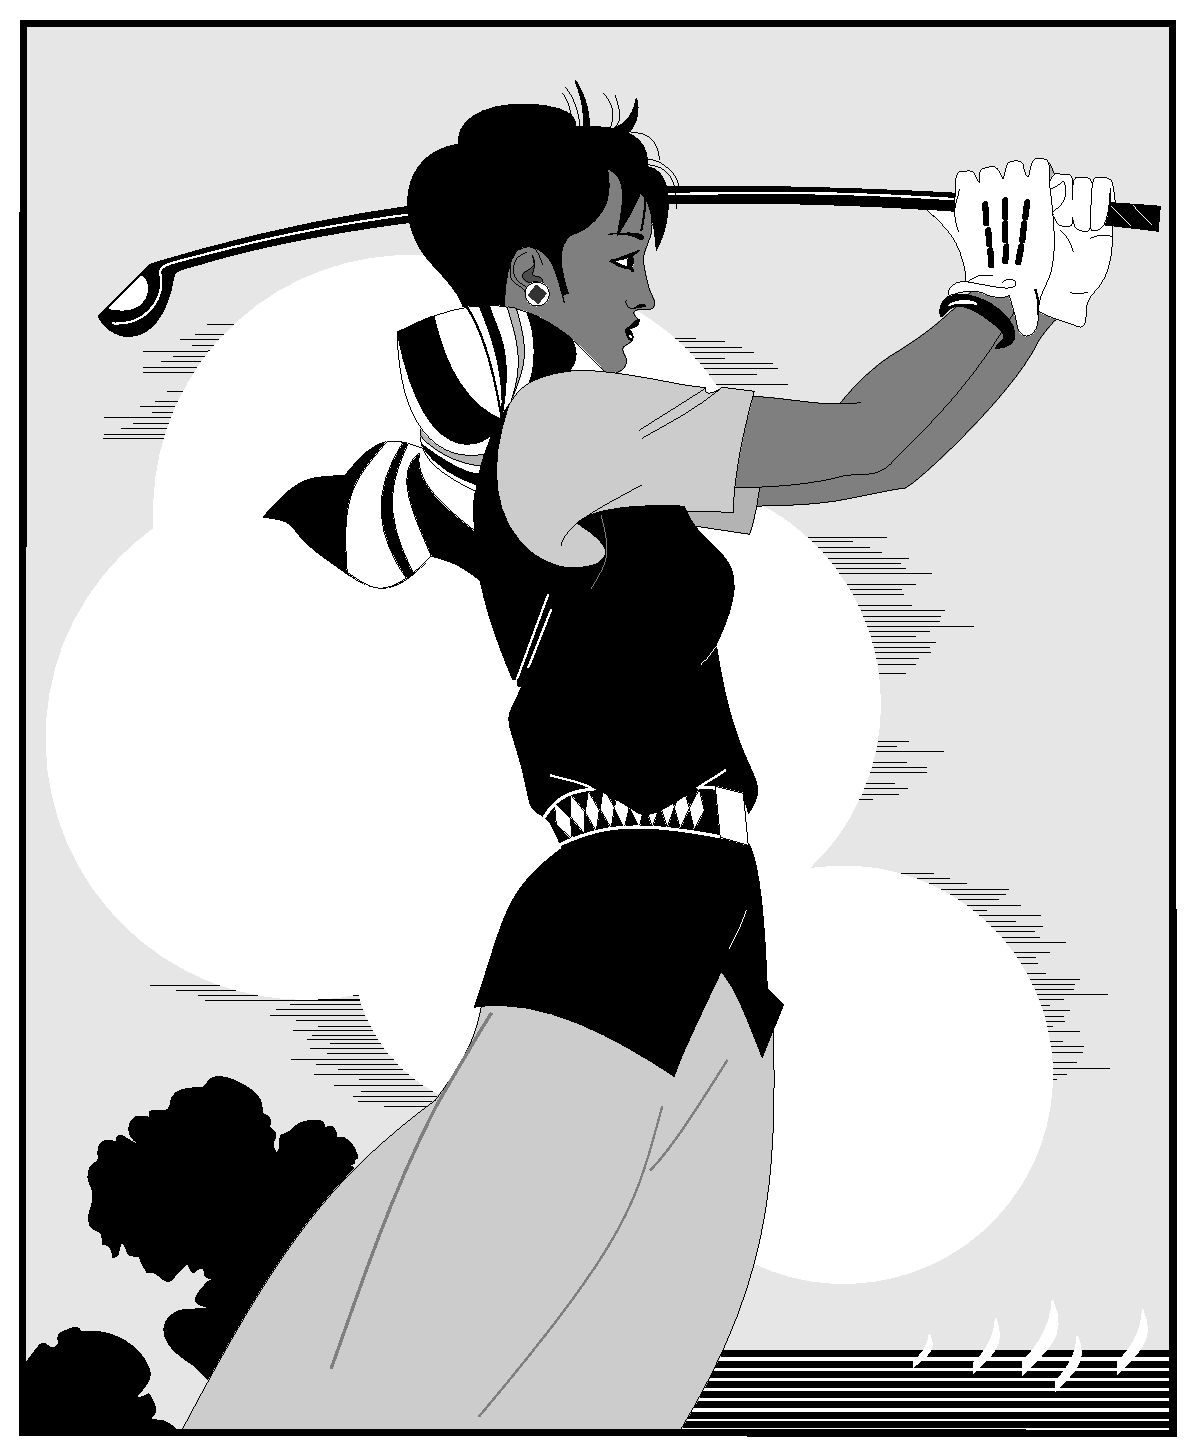
\includegraphics[width=\textwidth,height=\textwidth]{golfer}
\bicaption[golfer9]{}{打高尔夫球的人。注意,此图对齐方式是图片底部对齐}{Fig.$\!$}{The person playing golf. Please note that, it is vertically bottom aligned for figure.}
\end{minipage}
\centering
\begin{minipage}[t]{0.4\textwidth}
\centering
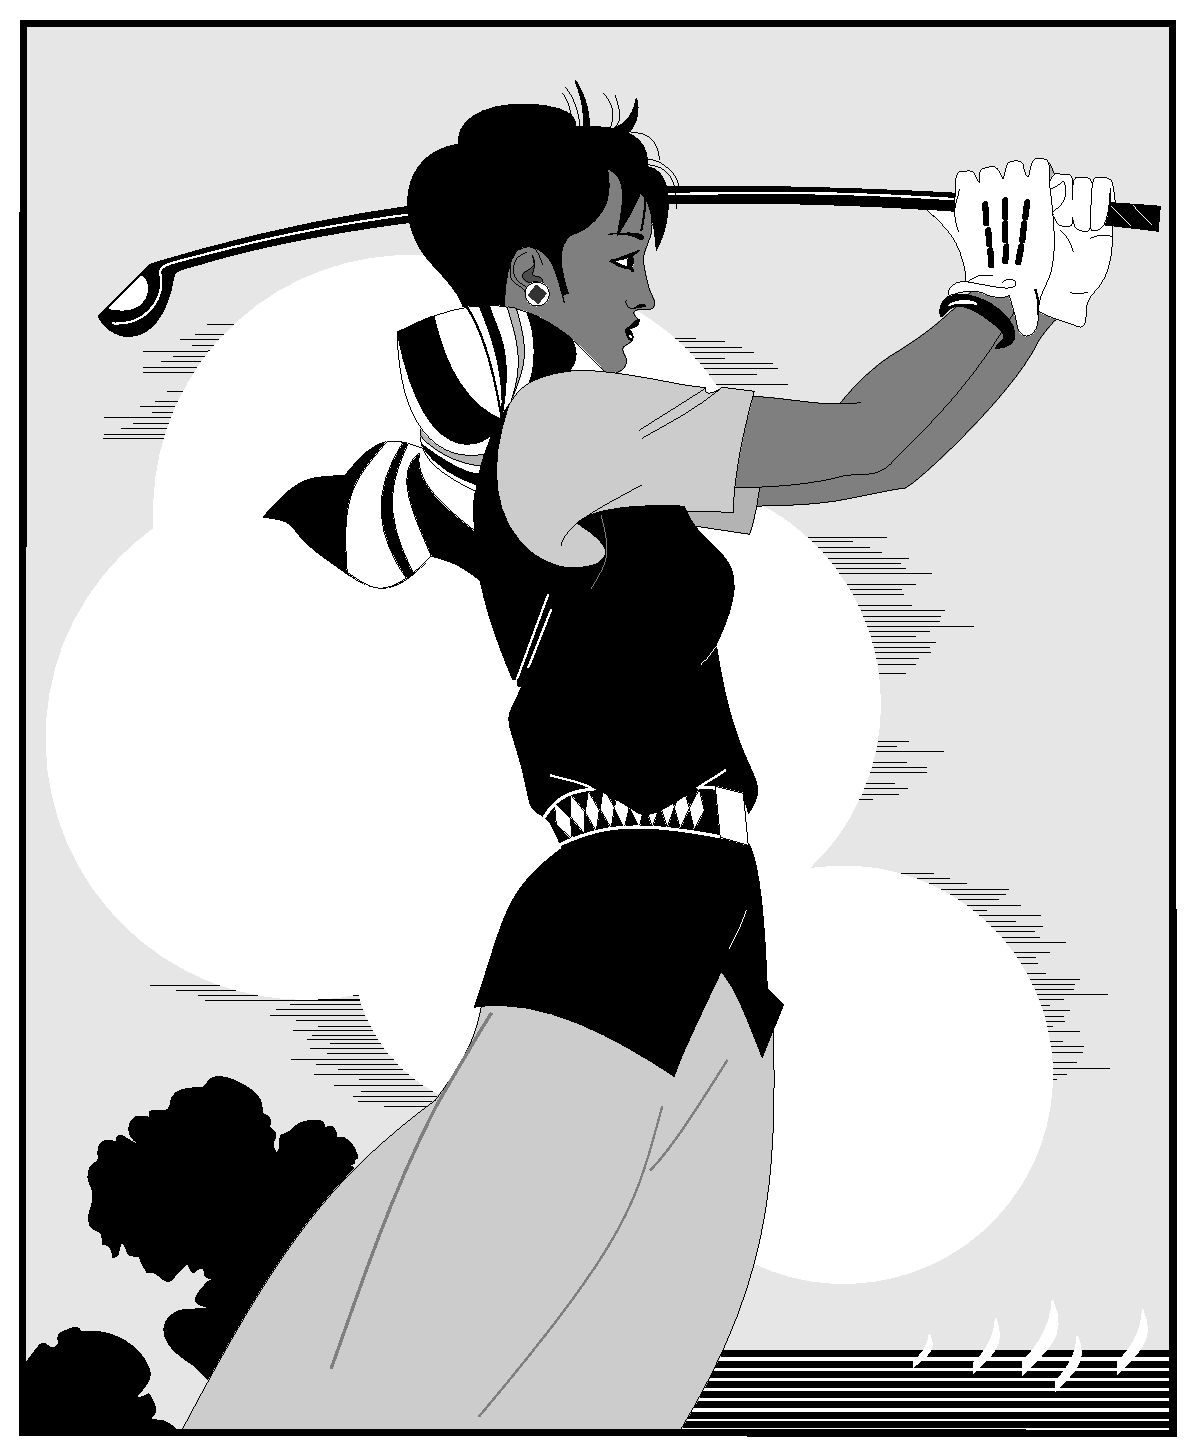
\includegraphics[width=\textwidth]{golfer}
\bicaption[golfer6]{}{打高尔夫球的人}{Fig.$\!$}{The person playing golf}
\end{minipage}
\end{figure}

\subsubsection{子图}[Sub-picture example]

注意:子图题注也可以只用中文。规范规定“分图题置于分图之下或图题之下”,但没有给出具体的格式要求。
没有要求的另外一个说法就是“无论什么格式都不对”。
所以只有在一个图中有标注“(a),(b)”,无法使用\cs{subfigure}的情况下,使用最后一个图例中的格式设置方法,否则不要使用。
为了应对“无论什么格式都不对”,这个子图图题使用“minipage”和“description”环境,宽度,对齐方式可以按照个人喜好自由设置,是否使用双语子图图题也可以自由设置。

\lipsum[1-3]

无意义文字,每页底部不要留空白。

\lipsum[4-5]

\begin{figure}[!ht]
\setlength{\subfigcapskip}{-1bp}
\centering
\begin{minipage}{\textwidth}
\centering
\subfigure{\label{golfer41}}\addtocounter{subfigure}{-2}
\subfigure[The person playing golf]{\subfigure[打高尔夫球的人~1]{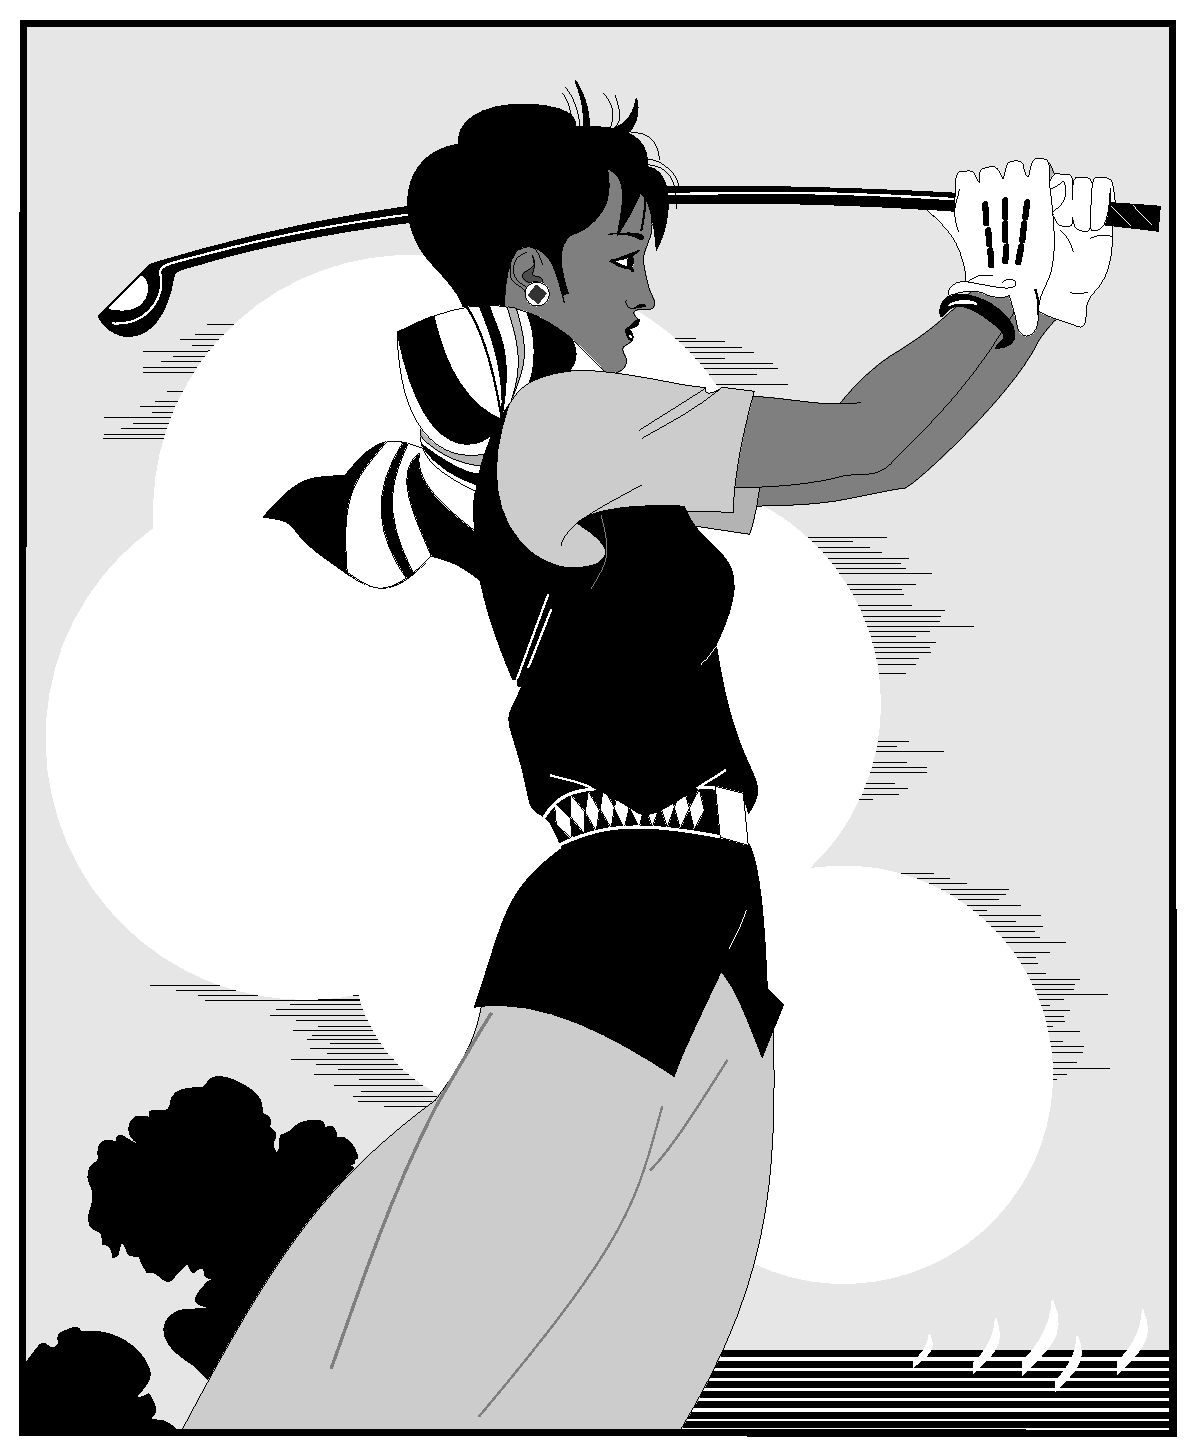
\includegraphics[width=0.4\textwidth]{golfer}}}
\hspace{2em}
\subfigure{\label{golfer42}}\addtocounter{subfigure}{-2}
\subfigure[The person playing golf]{\subfigure[打高尔夫球的人~2]{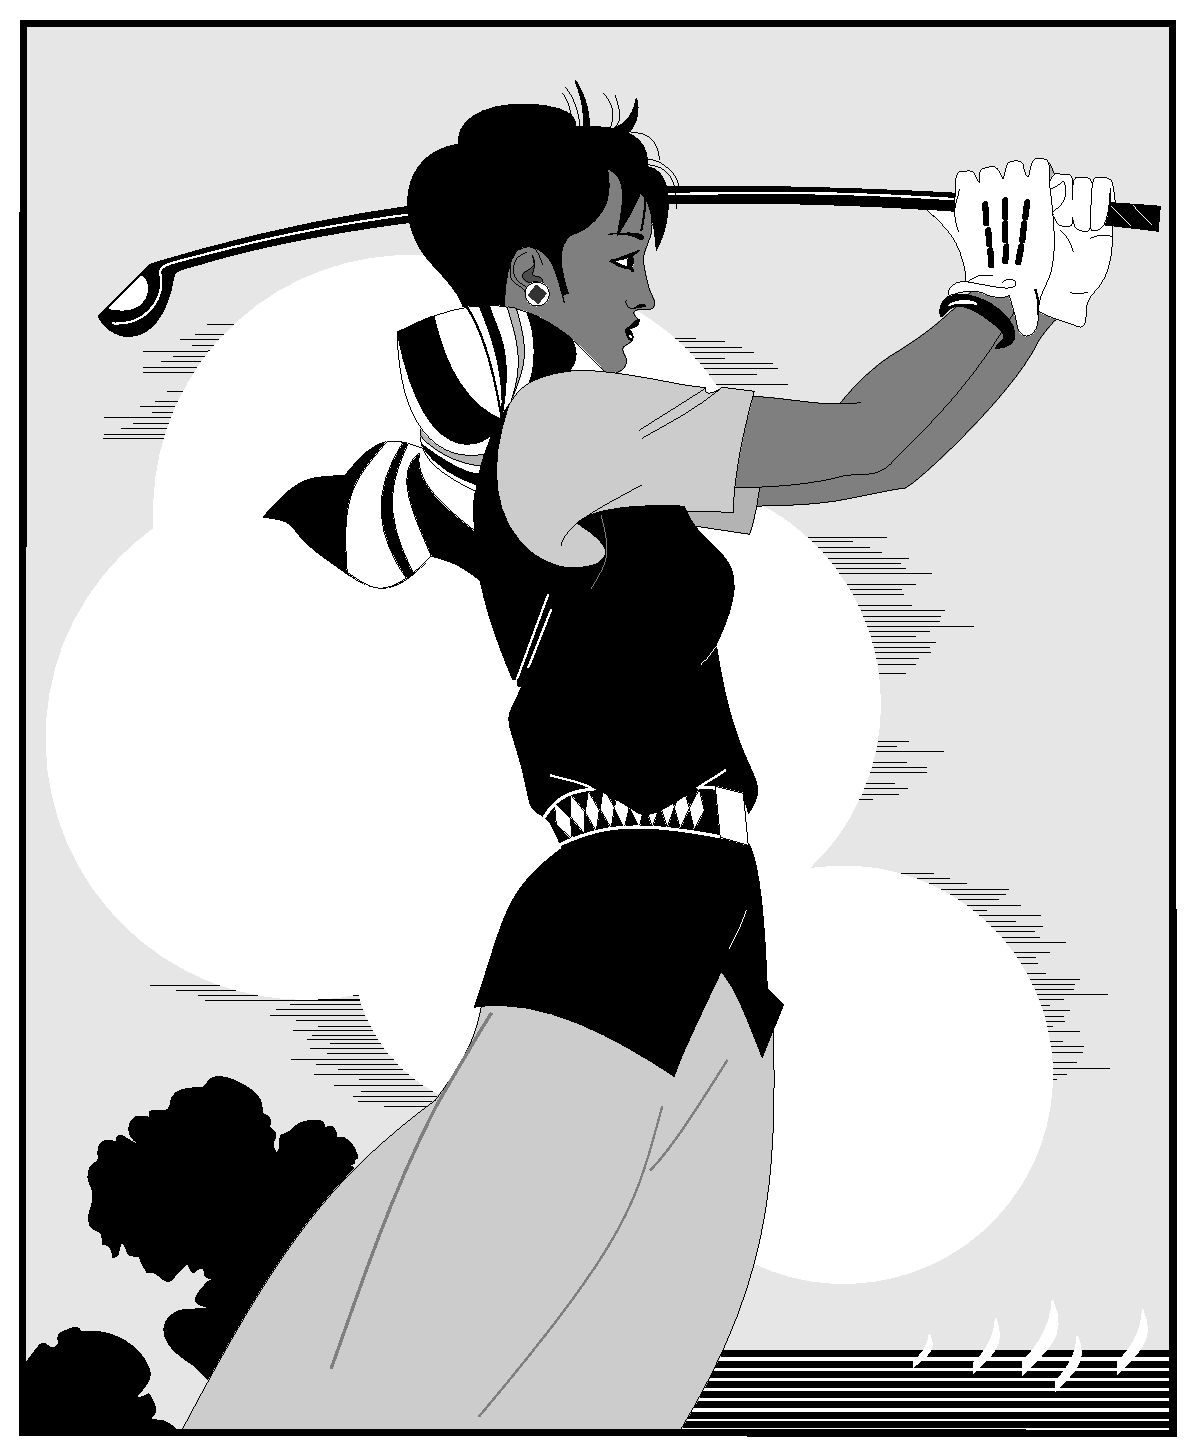
\includegraphics[width=0.4\textwidth]{golfer}}}
\end{minipage}
\centering
\begin{minipage}{\textwidth}
\centering
\subfigure{\label{golfer43}}\addtocounter{subfigure}{-2}
\subfigure[The person playing golf]{\subfigure[打高尔夫球的人~3]{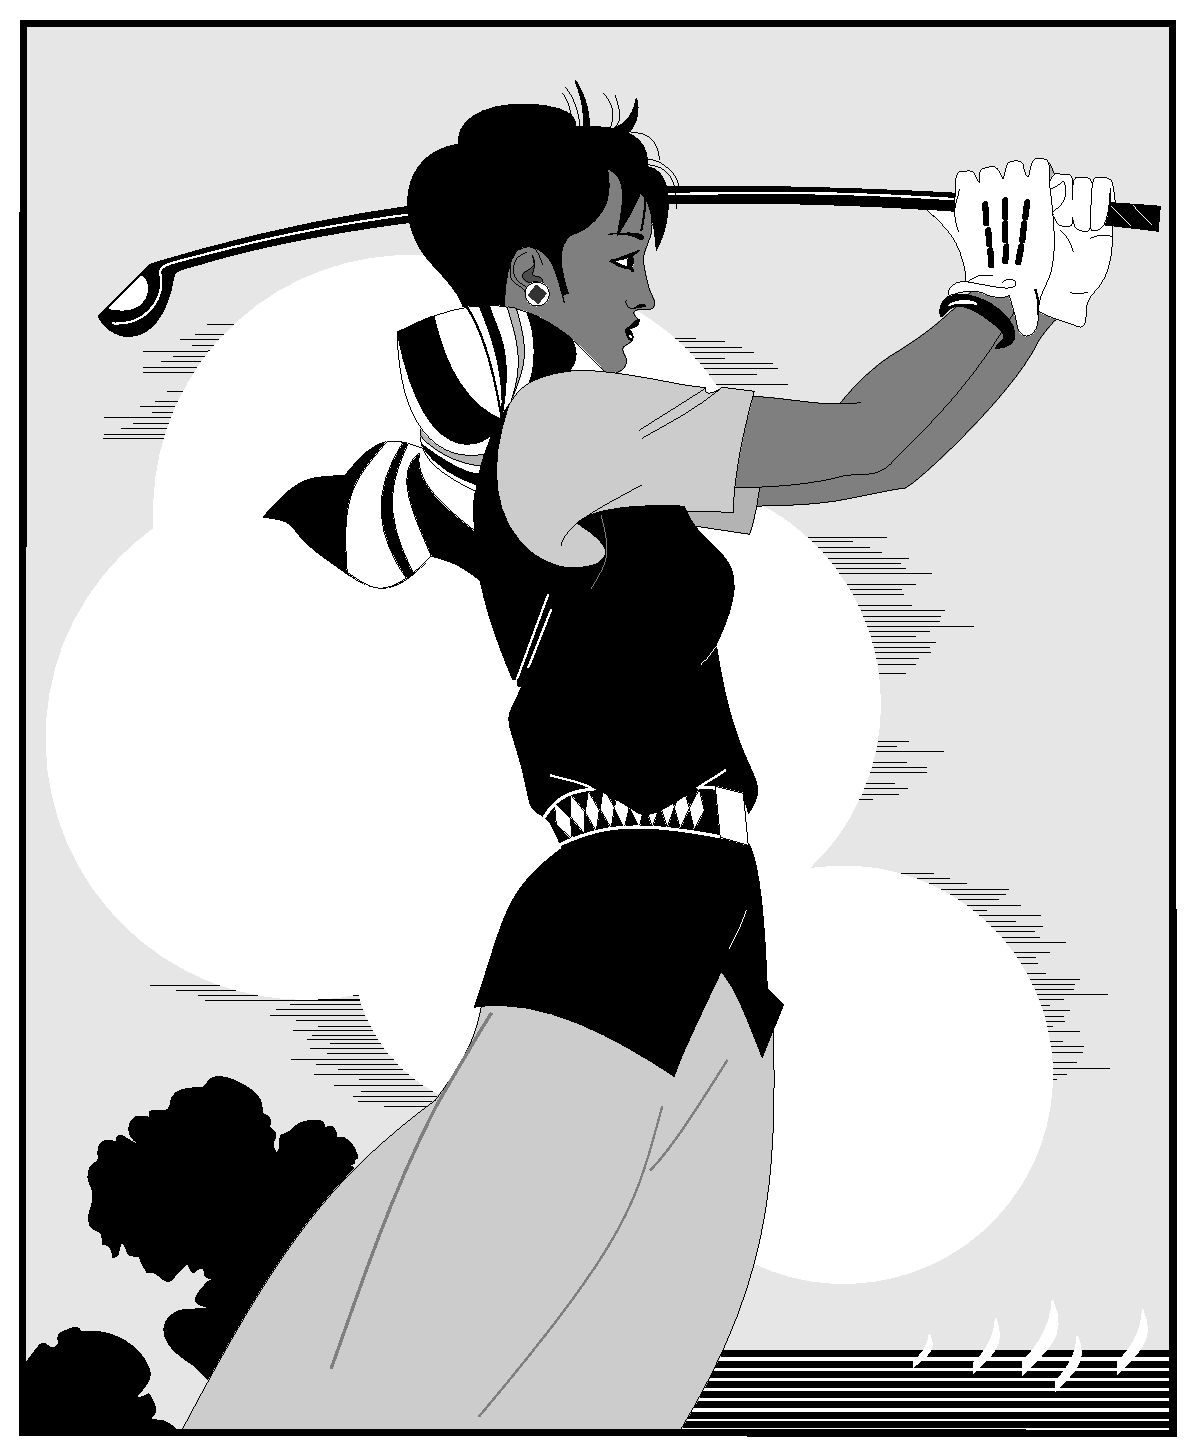
\includegraphics[width=0.4\textwidth]{golfer}}}
\hspace{2em}
\subfigure{\label{golfer44}}\addtocounter{subfigure}{-2}
\subfigure[The person playing golf. Here, 'hang indent' and 'center last line' are not stipulated in the regulation.]{\subfigure[打高尔夫球的人~4。注意,规范中没有明确规定要悬挂缩进、最后一行居中。]{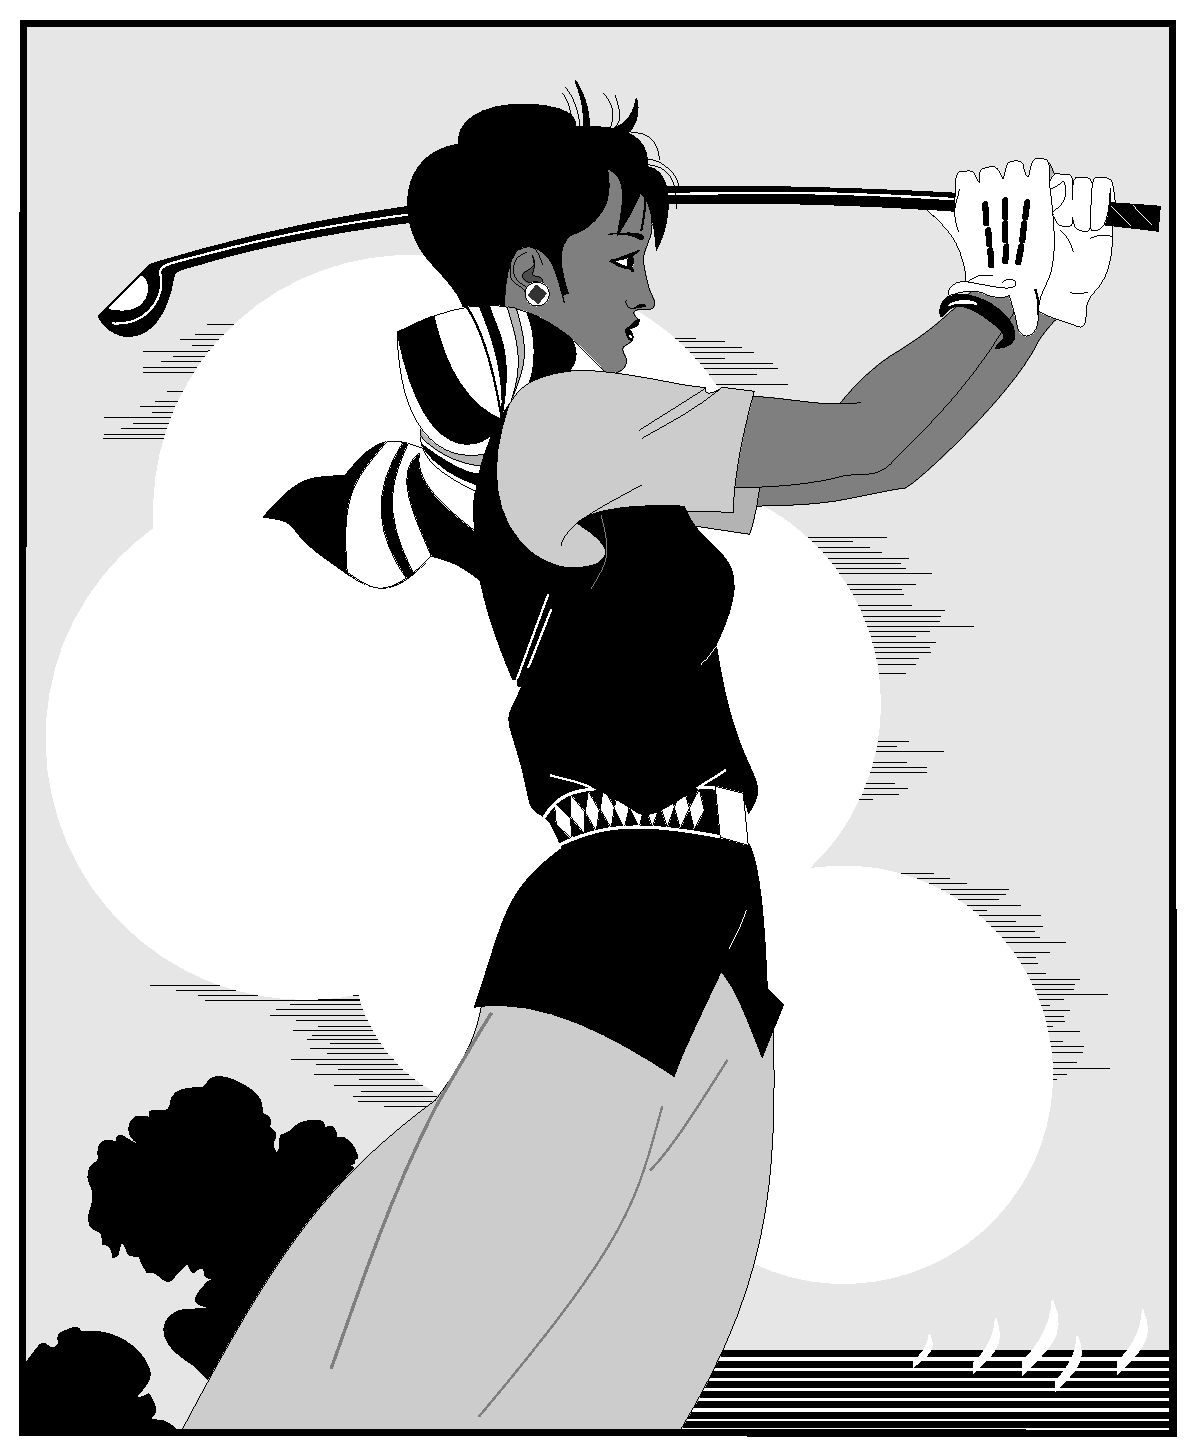
\includegraphics[width=0.4\textwidth]{golfer}}}
\end{minipage}
\vspace{0.2em}
\bicaption[golfer4]{}{打高尔夫球的人}{Fig.$\!$}{The person playing gol}
\end{figure}

\begin{figure}[t]
  \centering
  \begin{minipage}{.7\linewidth}
    \setlength{\subfigcapskip}{-1bp}
    \centering
    \begin{minipage}{\textwidth}
      \centering
      \subfigure{\label{golfer45}}\addtocounter{subfigure}{-2}
      \subfigure[The person playing golf]{\subfigure[打高尔夫球的人~1]{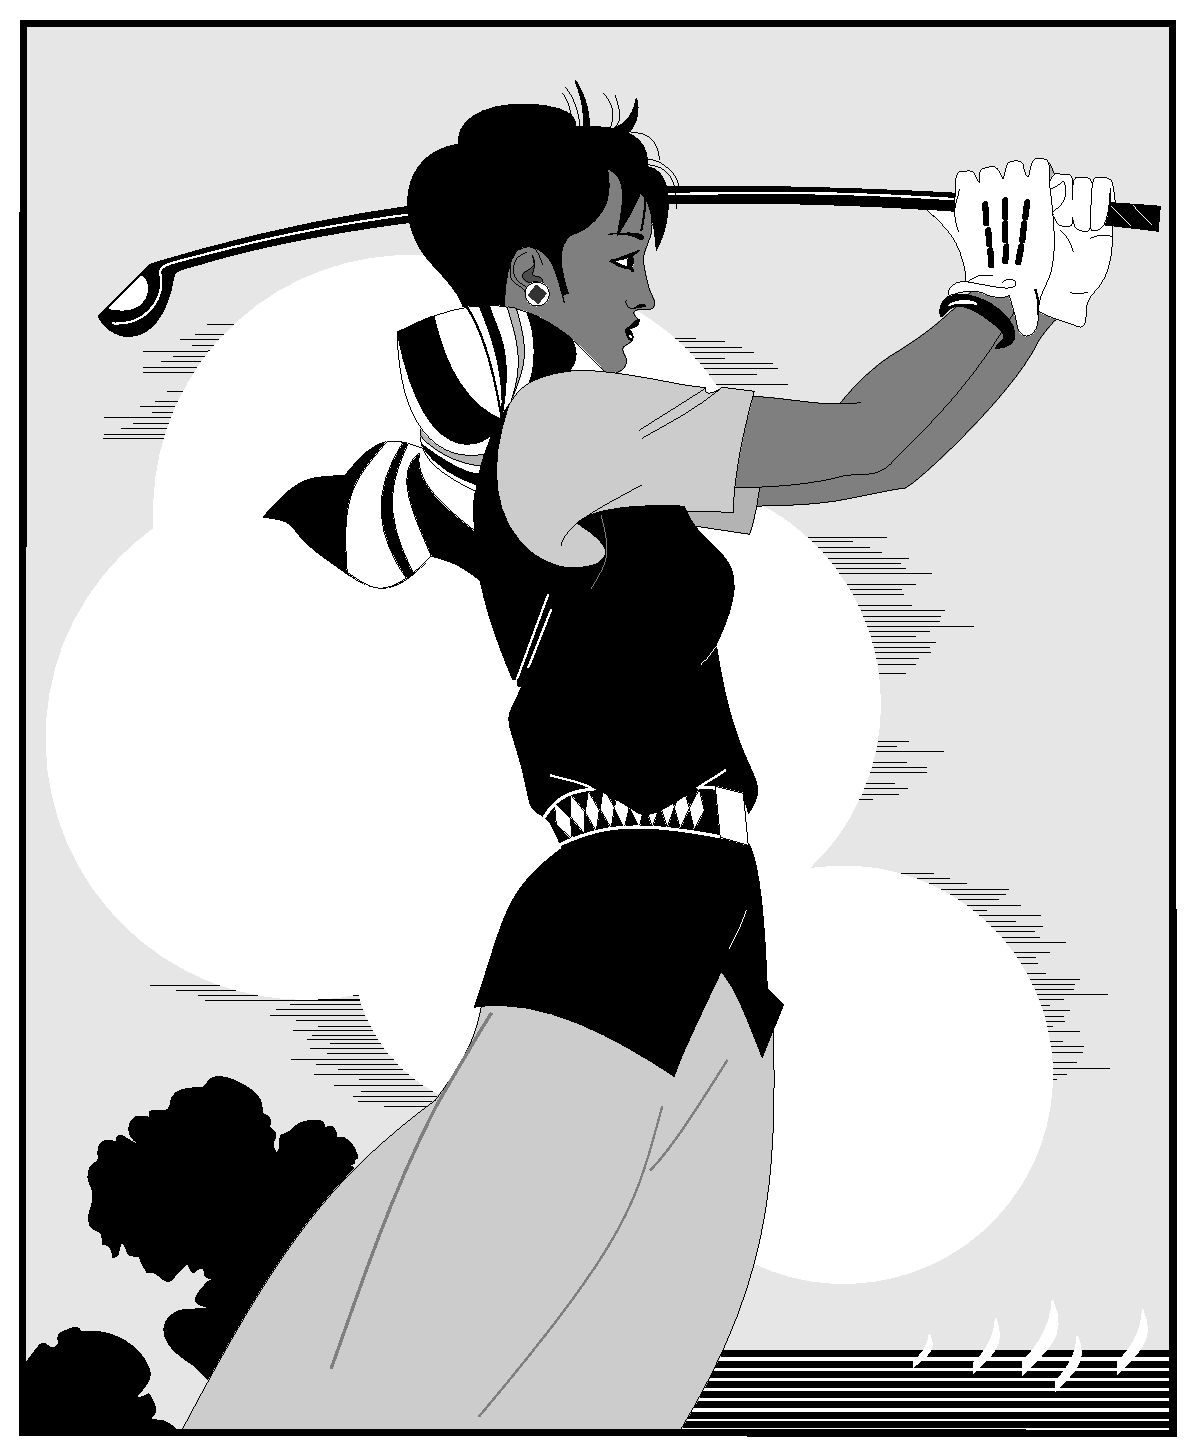
\includegraphics[width=0.4\textwidth]{golfer}}}
      \hspace{4em}
      \subfigure{\label{golfer46}}\addtocounter{subfigure}{-2}
      \subfigure[The person playing golf]{\subfigure[打高尔夫球的人~2]{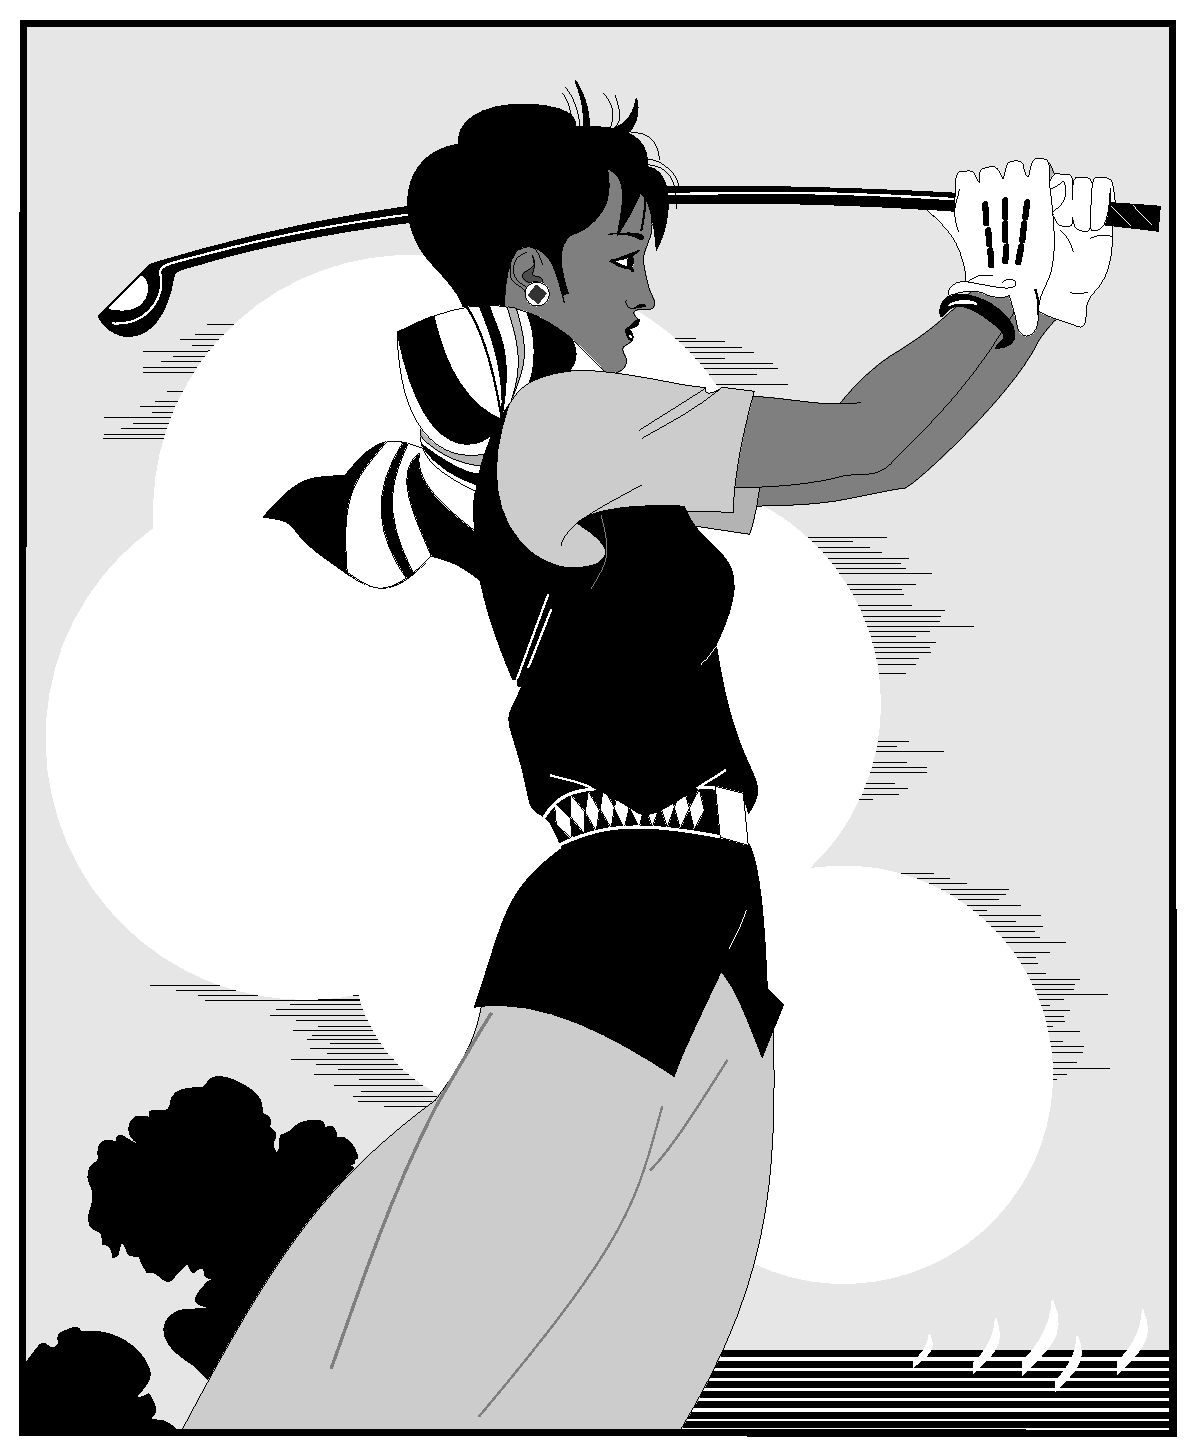
\includegraphics[width=0.4\textwidth]{golfer}}}
    \end{minipage}
    \vskip 0.2em
  \wuhao 注意:这里是中文图注添加位置(我工要求,图注在图题之上)。
    \vspace{0.2em}
\bicaption[golfer47]{}{打高尔夫球的人。注意,此处我工有另外一处要求,子图图题可以位于主图题之下。但由于没有明确说明位于下方具体是什么格式,所以这里不给出举例。}{Fig.$\!$}{The person playing golf. Please note that, although it is appropriate to put subfigures' captions under this caption as stipulated in regulation, but its format is not clearly stated.}
  \end{minipage}
\end{figure}

\begin{figure}[t]
\centering
% \begin{tikzpicture}
% 	\node[anchor=south west,inner sep=0] (image) at (0,0) {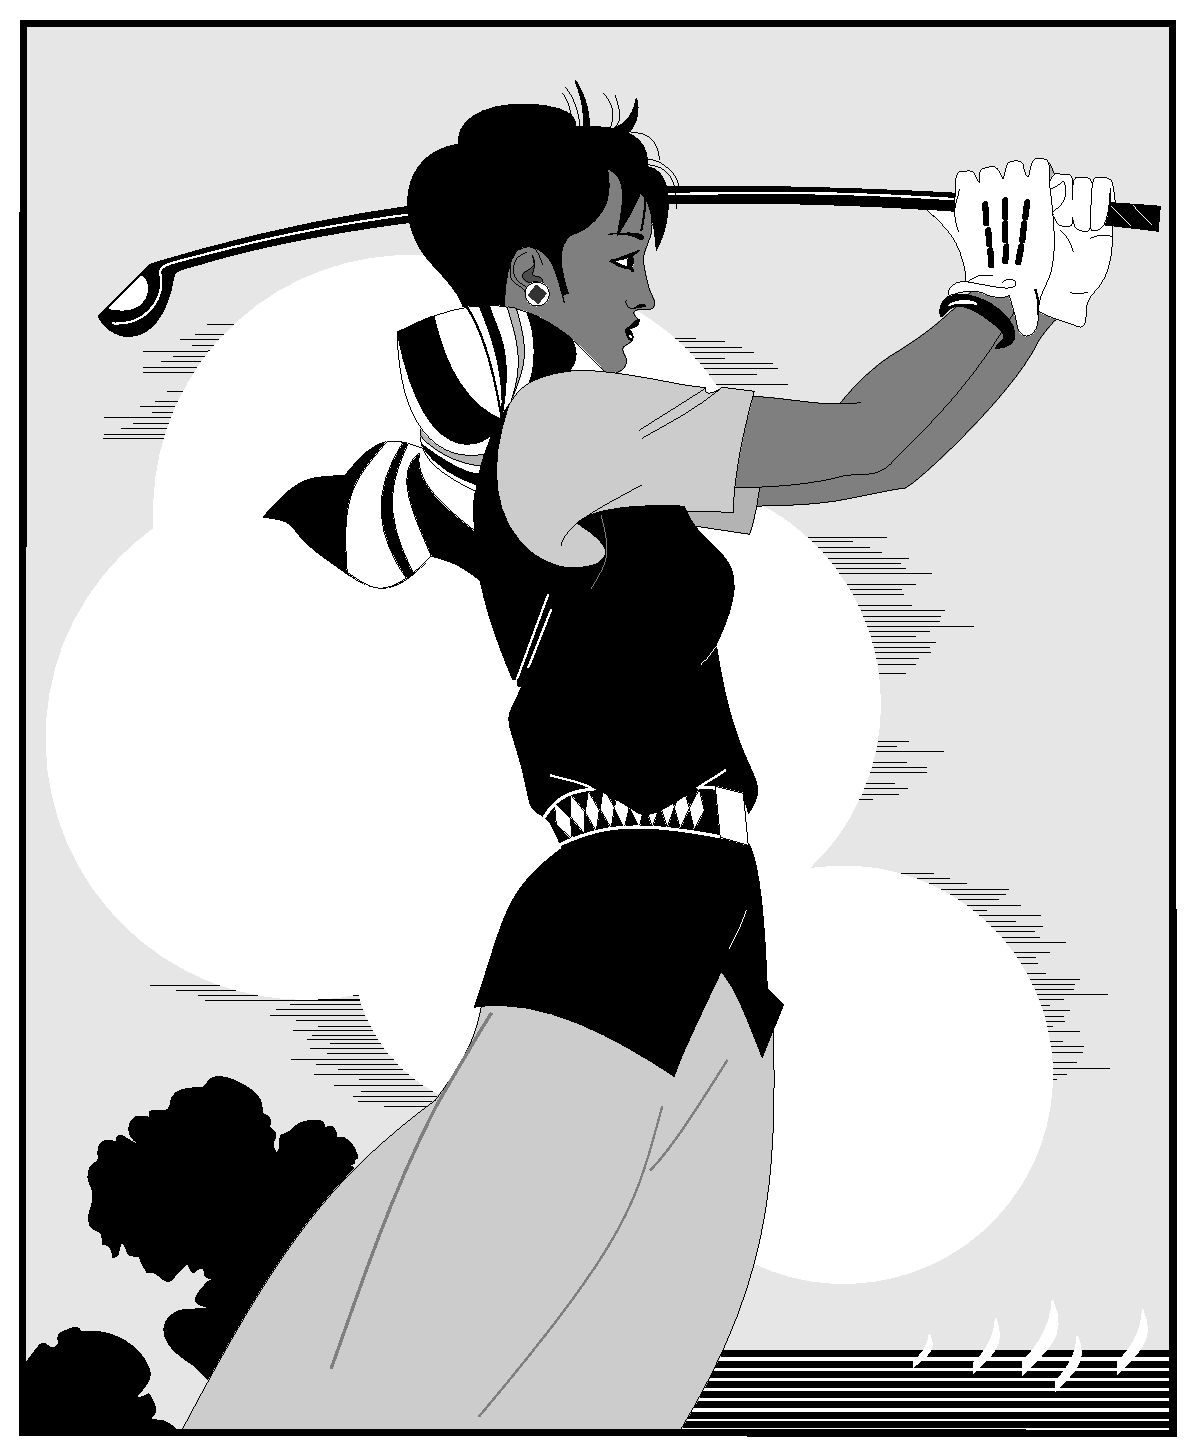
\includegraphics[width=0.3\textwidth]{golfer}};
% 	\begin{scope}[x={(image.south east)},y={(image.north west)}]
% 		\node at (0.3,0.5) {a)};
% 		\node at (0.8,0.2) {b)};
% 	\end{scope}
% \end{tikzpicture}
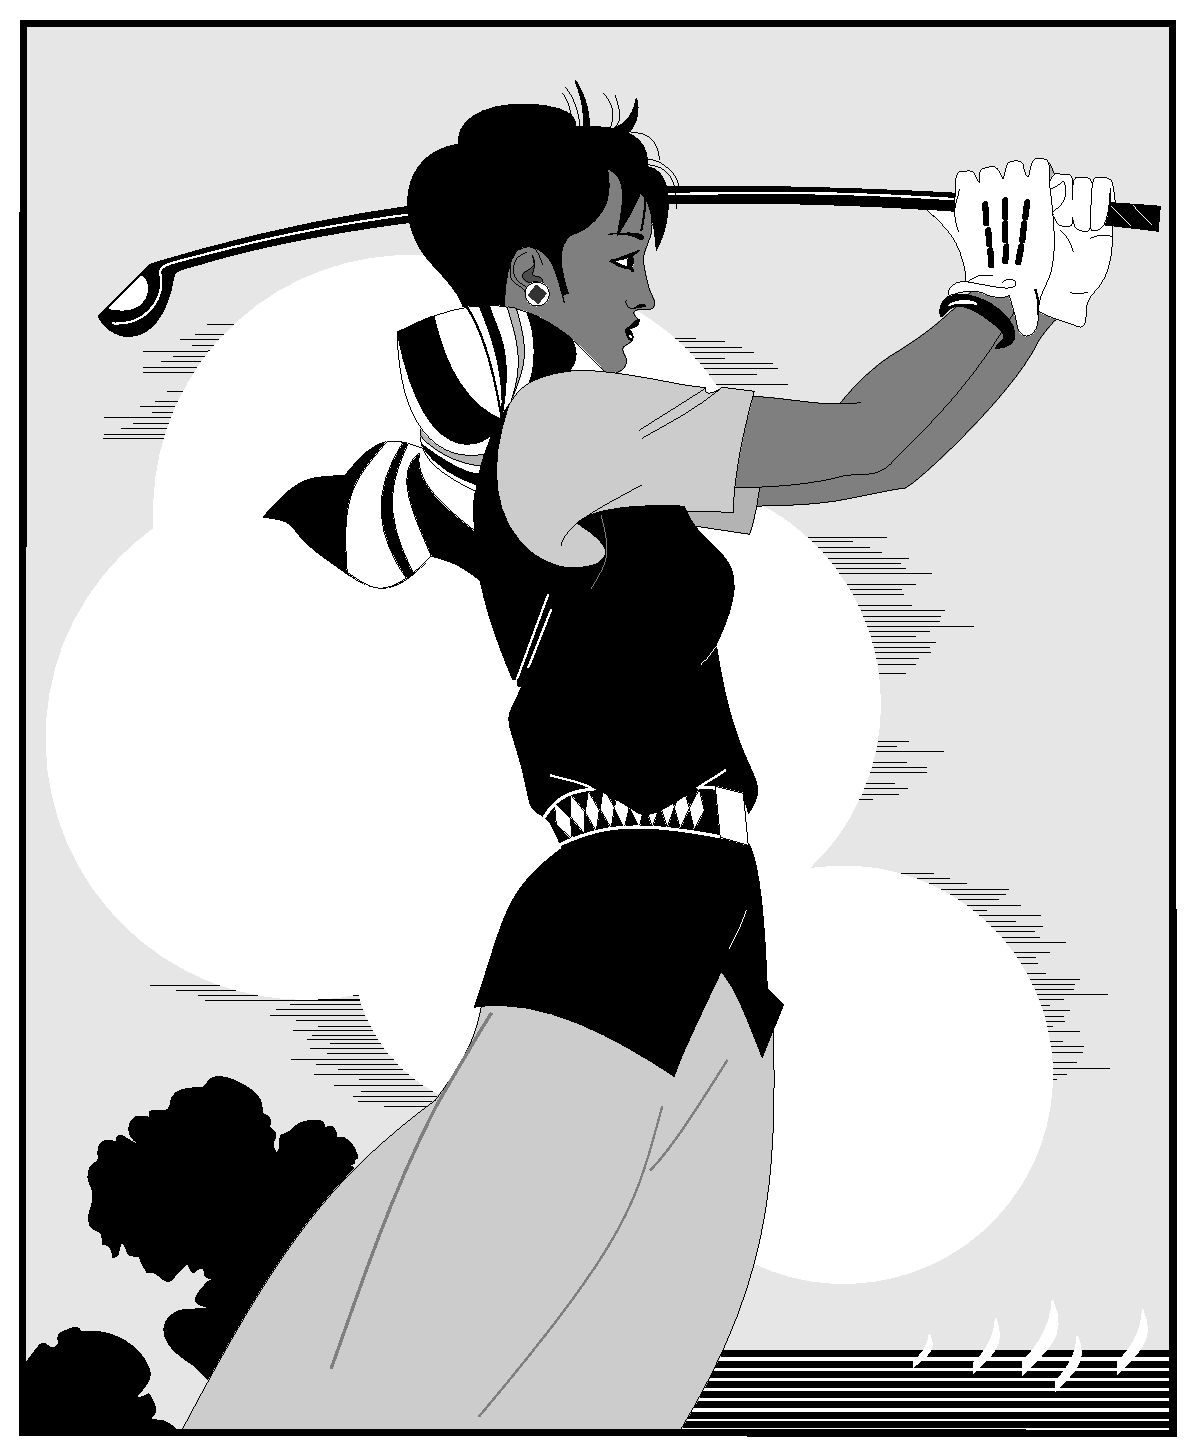
\includegraphics[width=0.3\textwidth]{golfer}
\bicaption[golfer0]{}{打高尔夫球球的人(博士论文双语题注)}{Fig.$\!$}{The person playing golf (Doctoral thesis)}
\vskip -0.4em
 \hspace{2em}
\begin{minipage}[t]{0.3\textwidth}
\wuhao \setlist[description]{font=\normalfont}
	\begin{description}
		\item[(a)]子图图题
		\item[(a)]Subfigure caption
	\end{description}
 \end{minipage}
 \hspace{2em}
 \begin{minipage}[t]{0.3\textwidth}
\wuhao \setlist[description]{font=\normalfont}
	\begin{description}
		\item[(b)]子图图题
		\item[(b)]Subfigure caption
	\end{description}
\end{minipage}
\end{figure}

\begin{figure}[!ht]
	\centering
	\begin{sideways}
		\begin{minipage}{\textheight}
			\centering
			\fbox{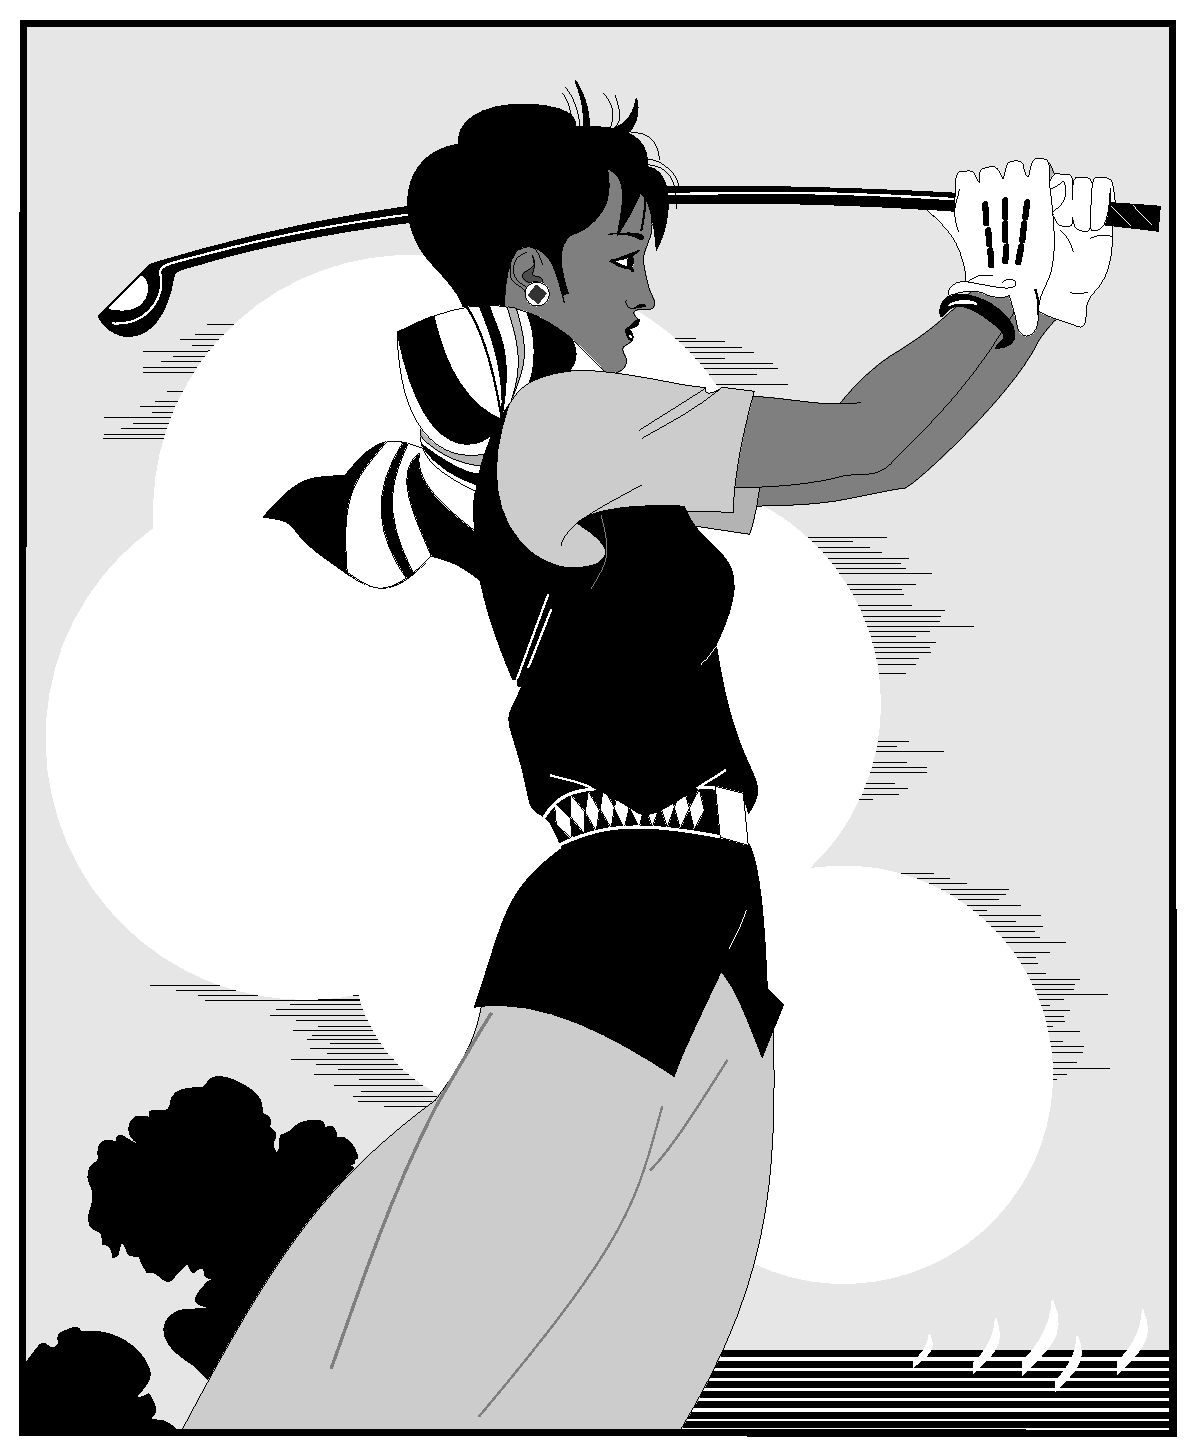
\includegraphics[width=0.2\textwidth]{golfer}}
			\fbox{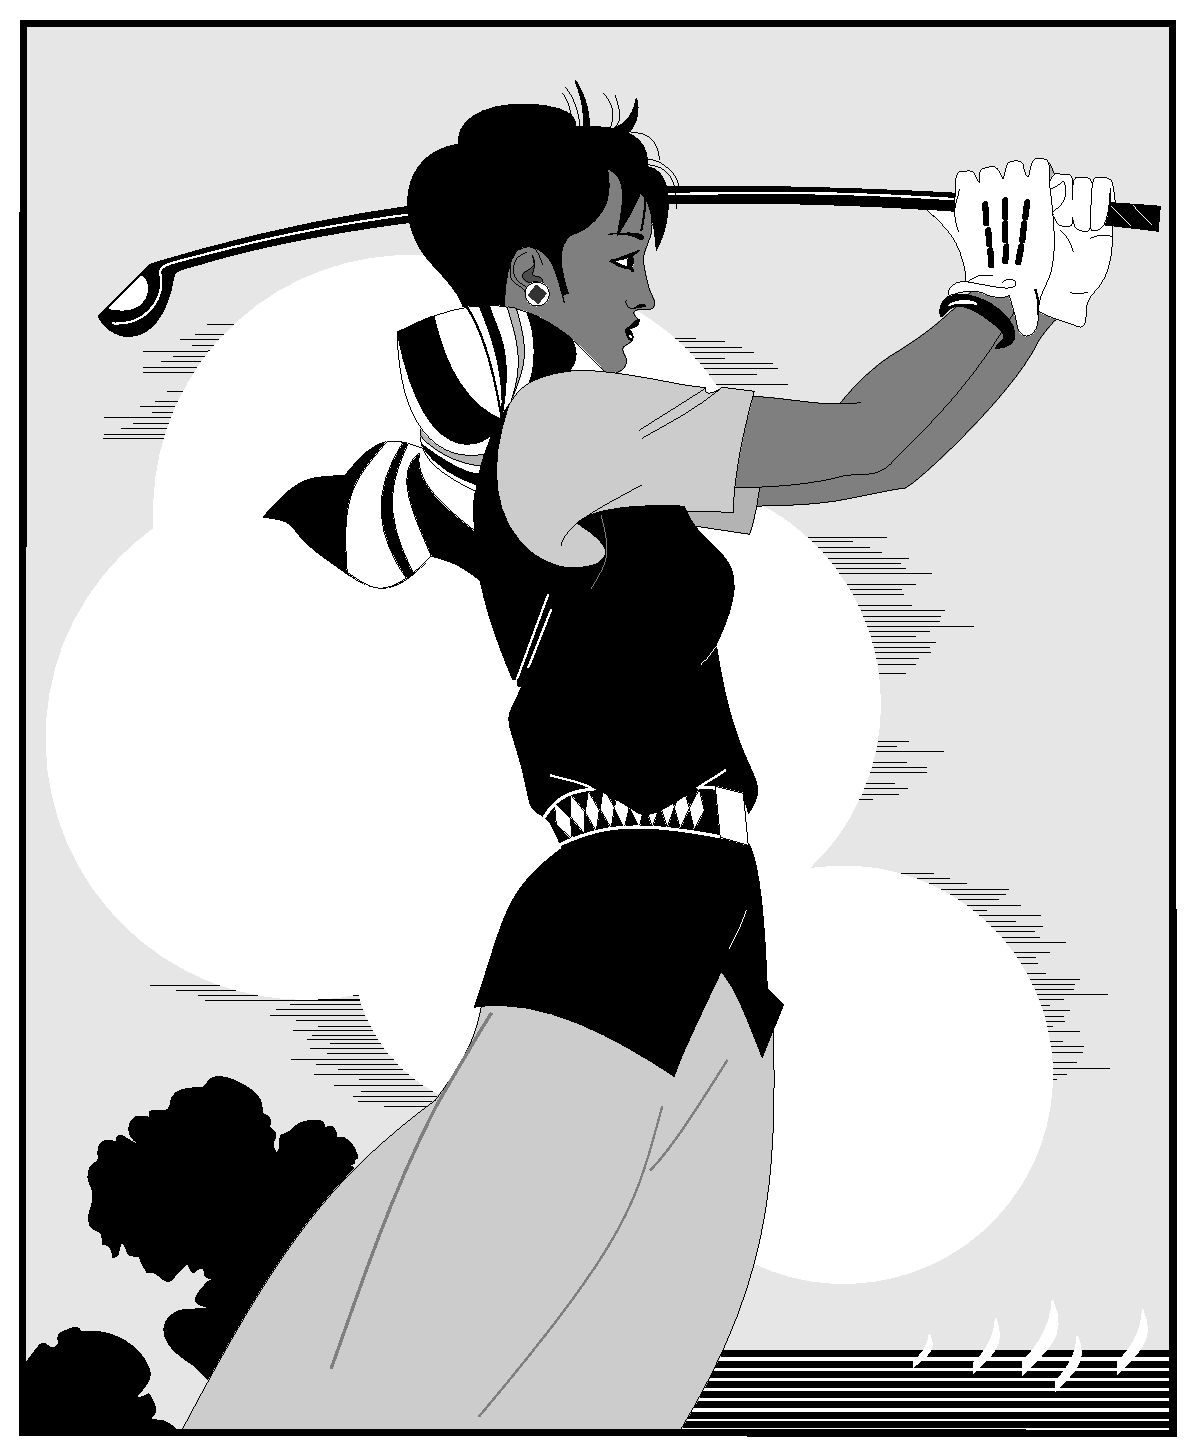
\includegraphics[width=0.2\textwidth]{golfer}}
			\fbox{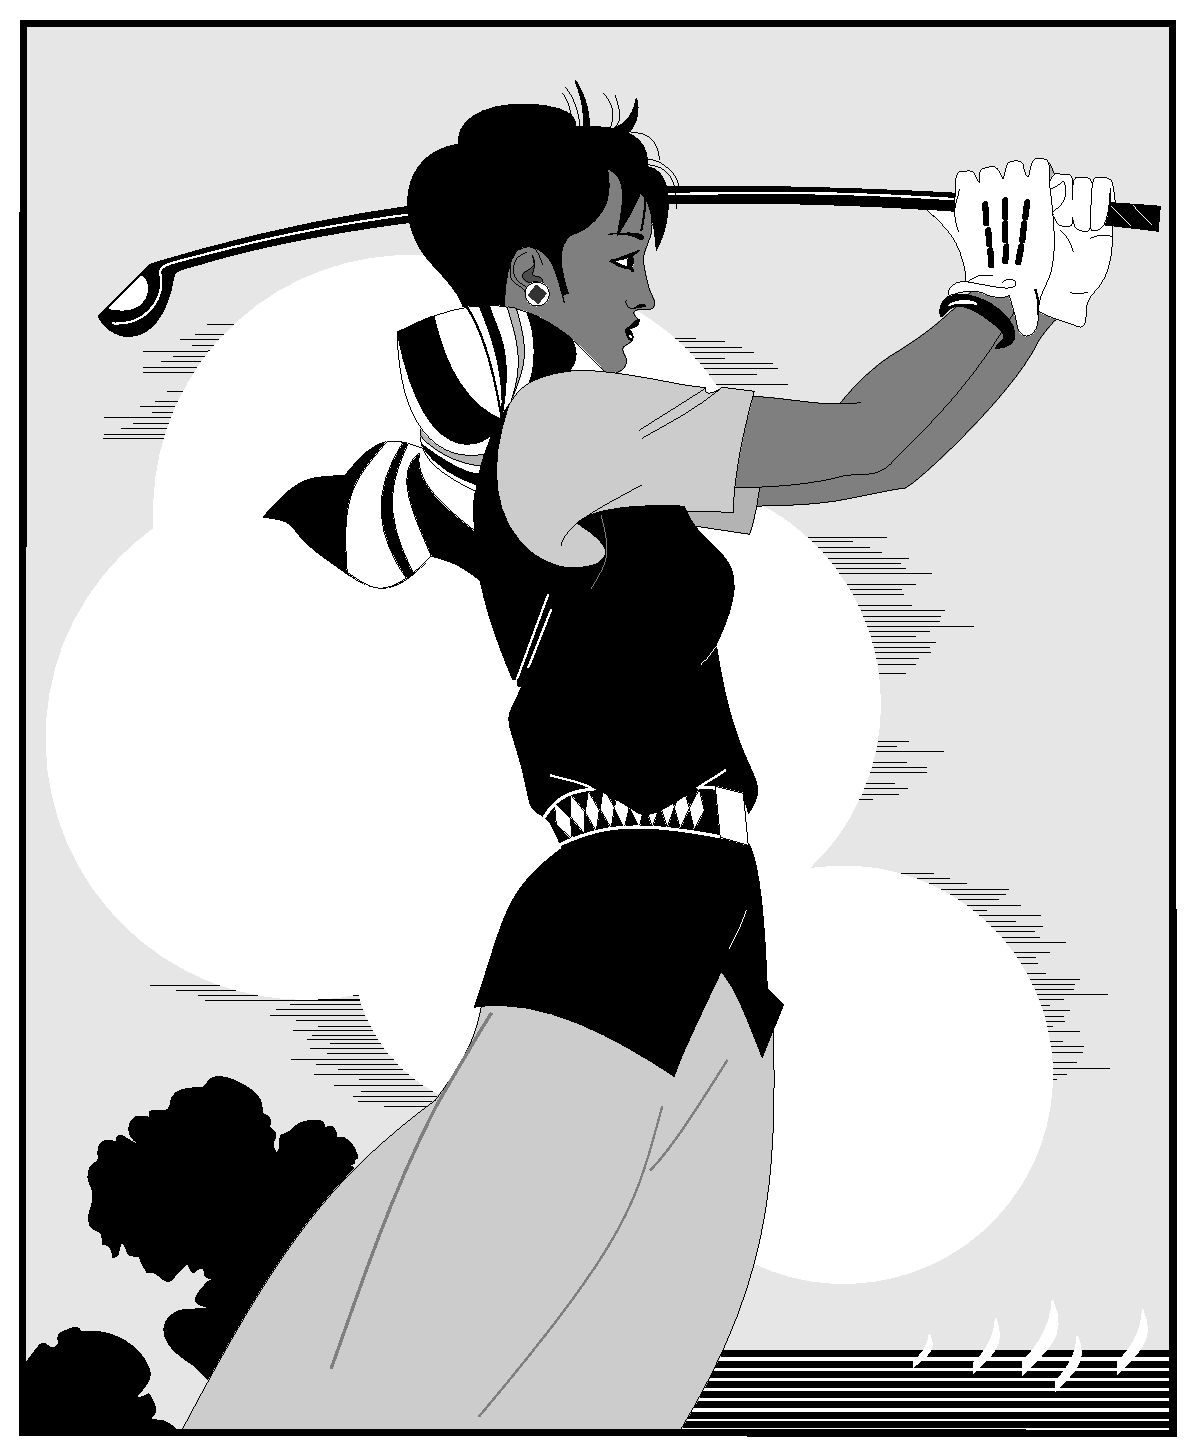
\includegraphics[width=0.2\textwidth]{golfer}}
			\fbox{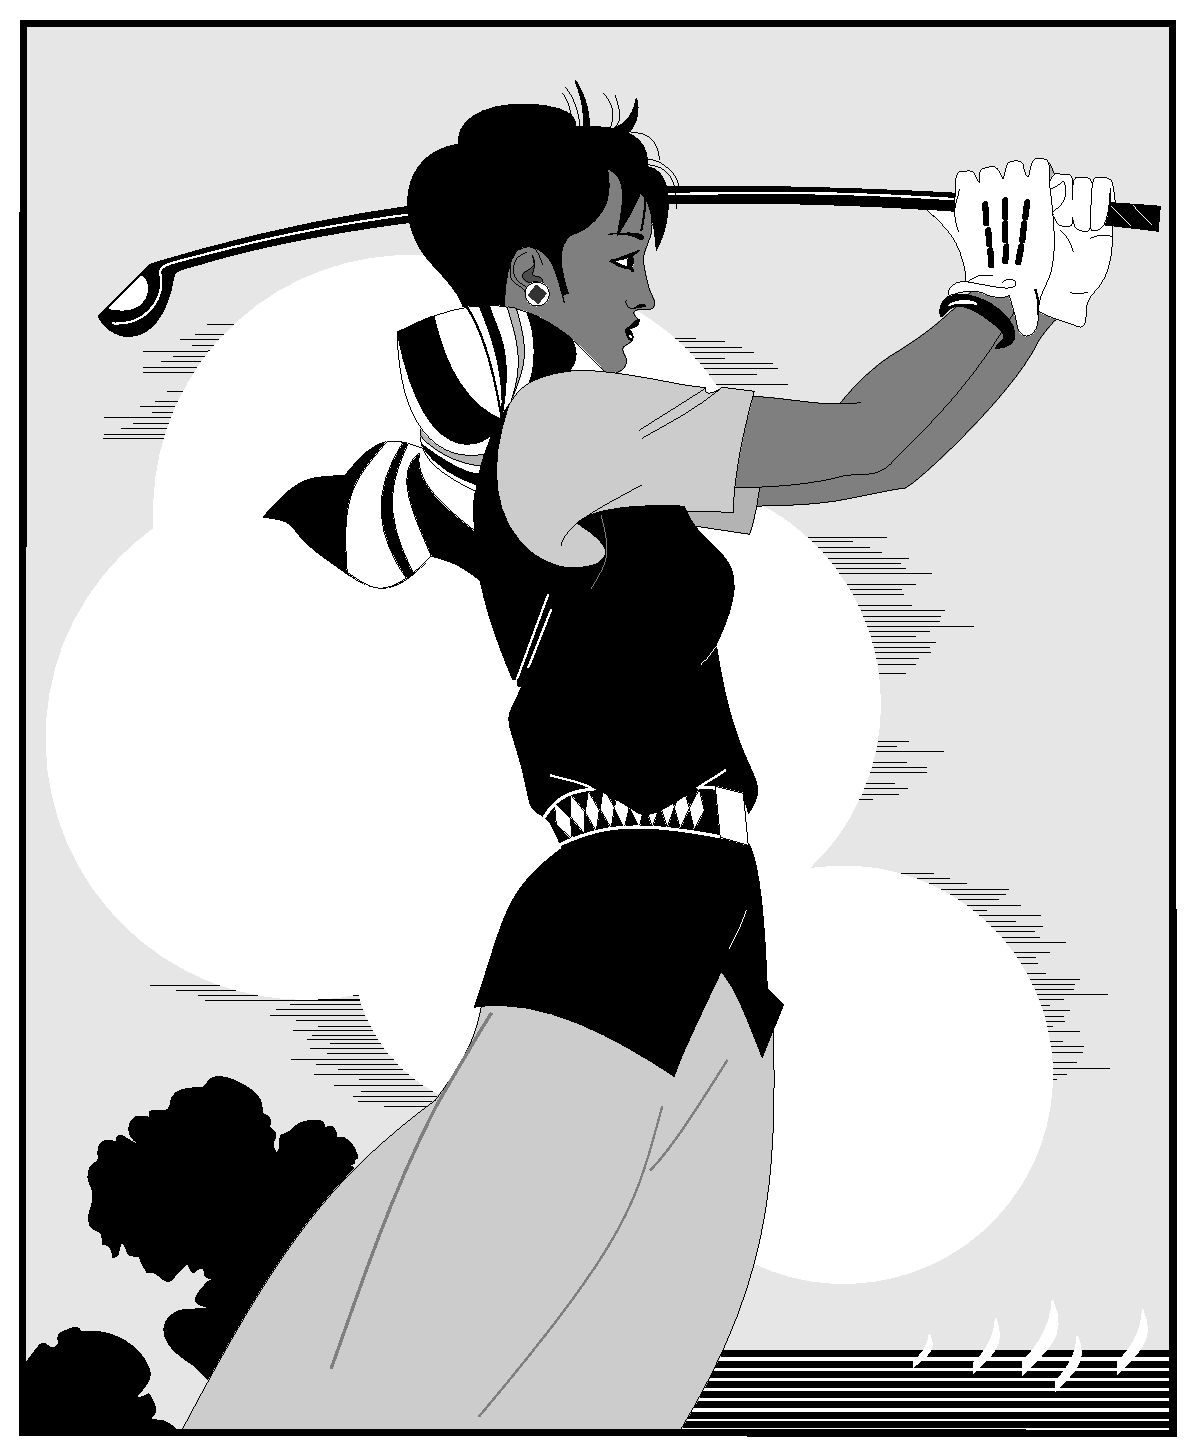
\includegraphics[width=0.2\textwidth]{golfer}}
			\fbox{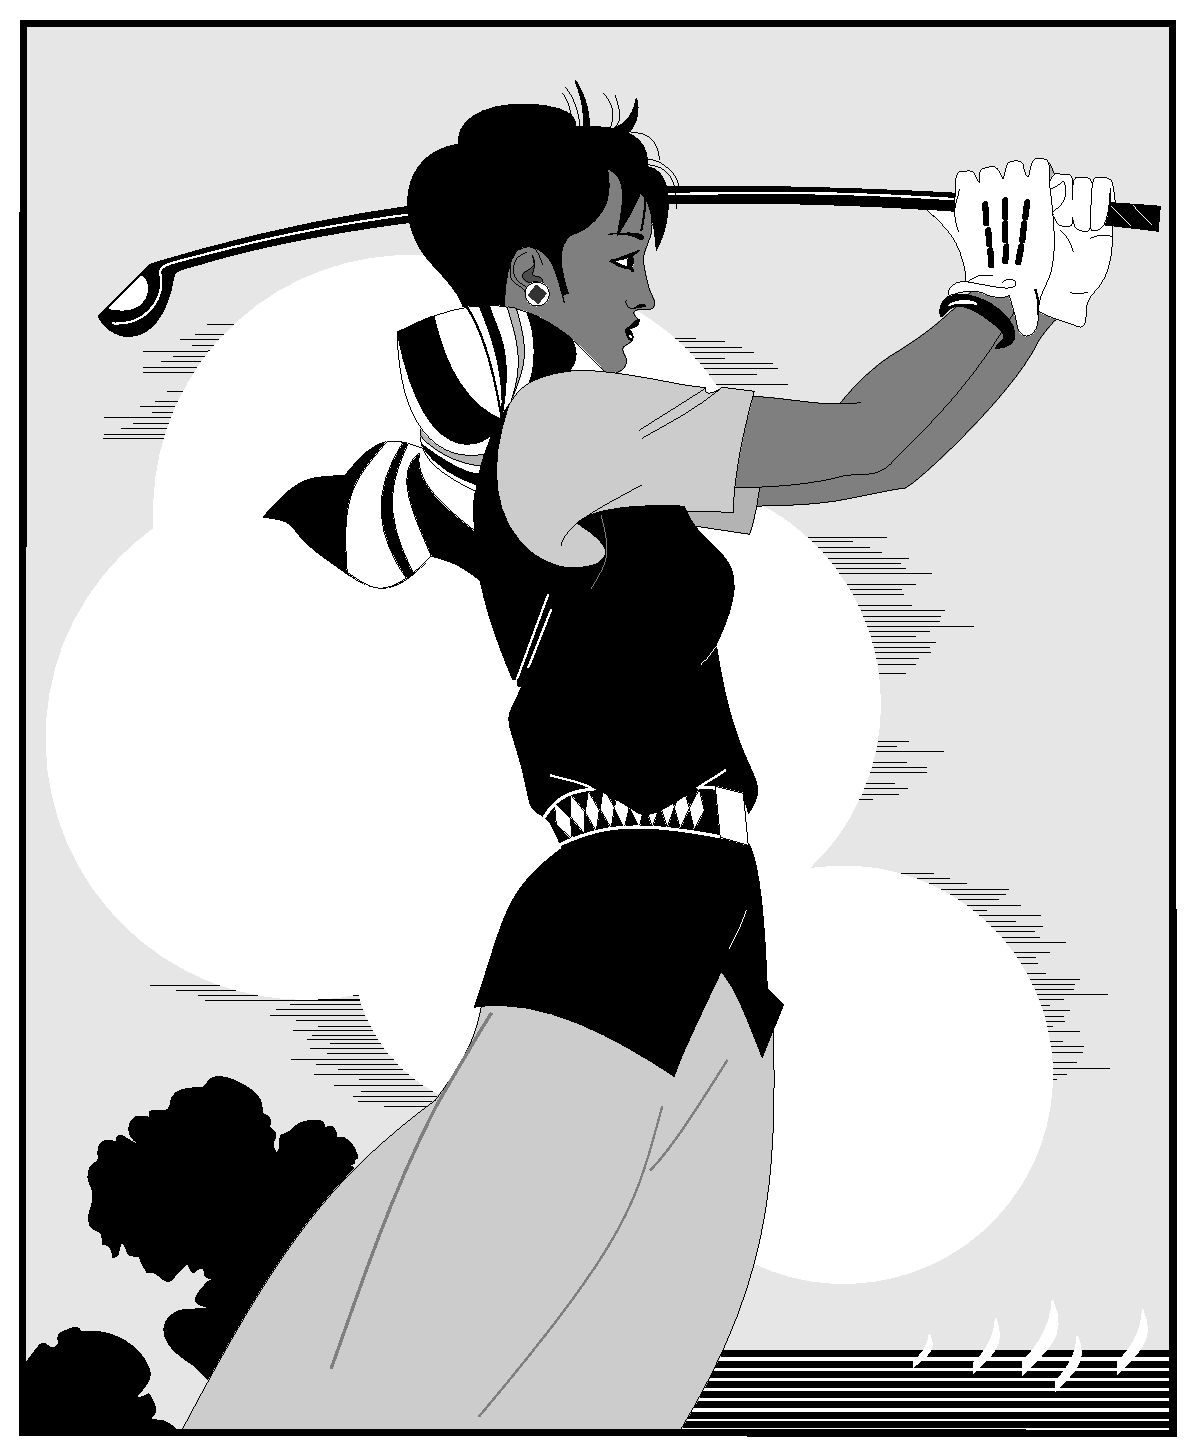
\includegraphics[width=0.2\textwidth]{golfer}}
			\fbox{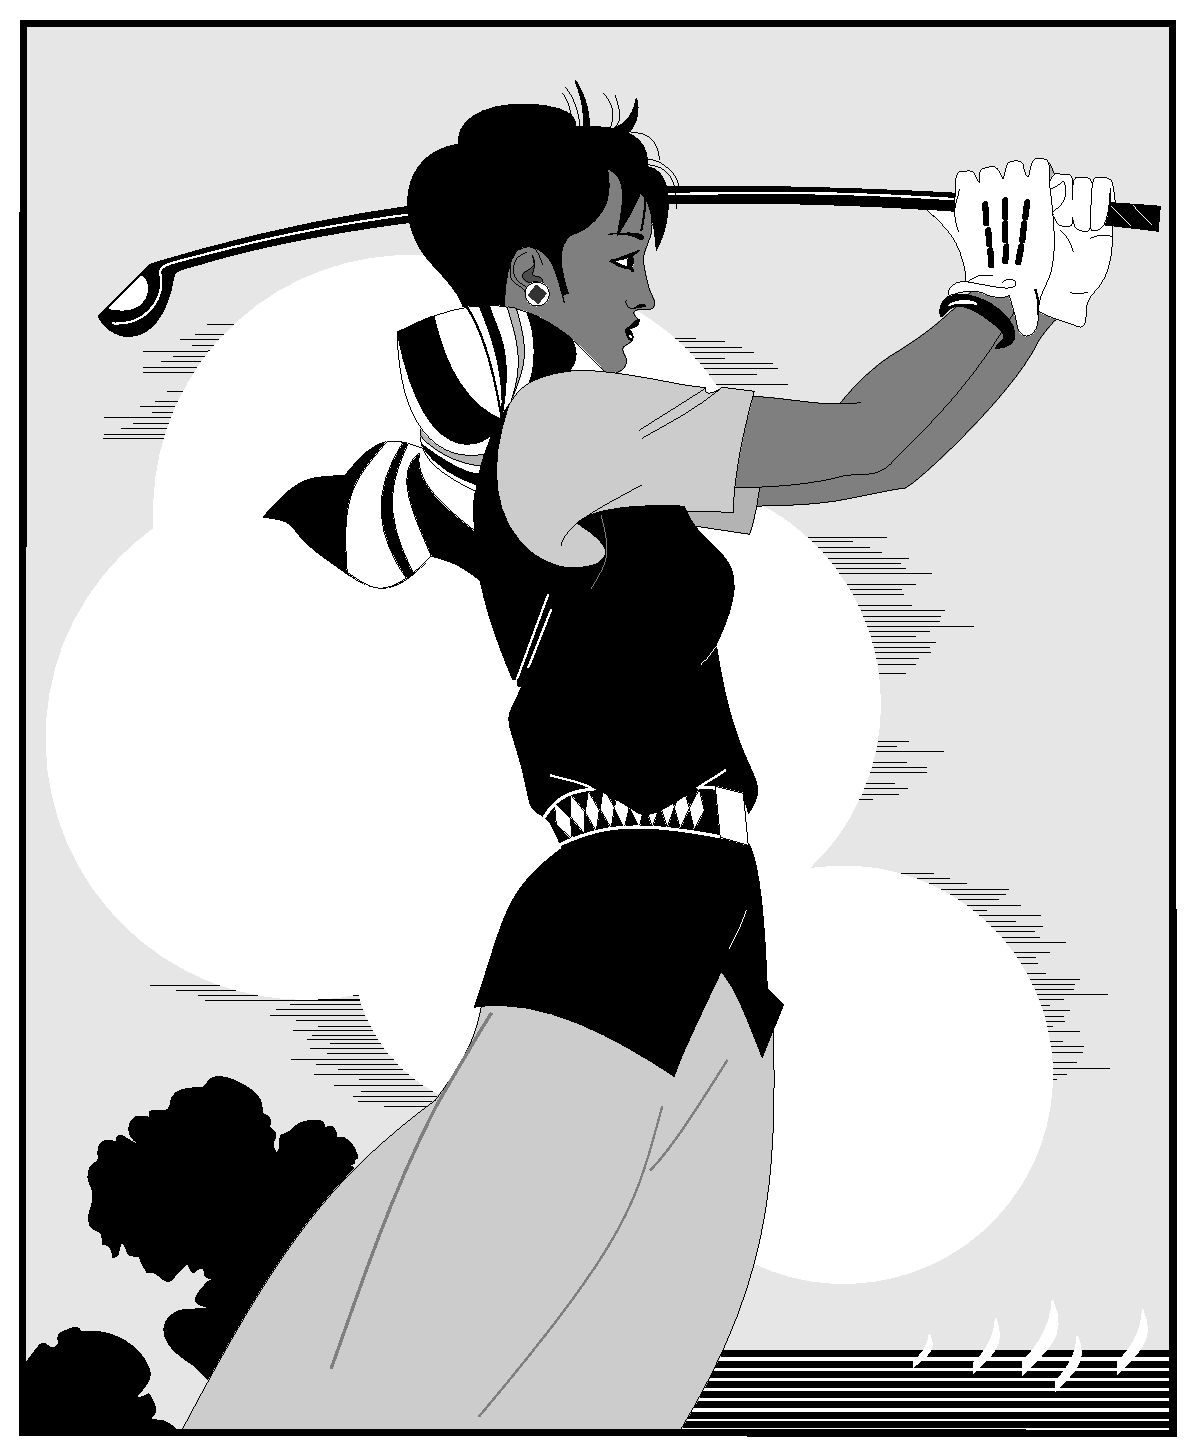
\includegraphics[width=0.2\textwidth]{golfer}}
			\fbox{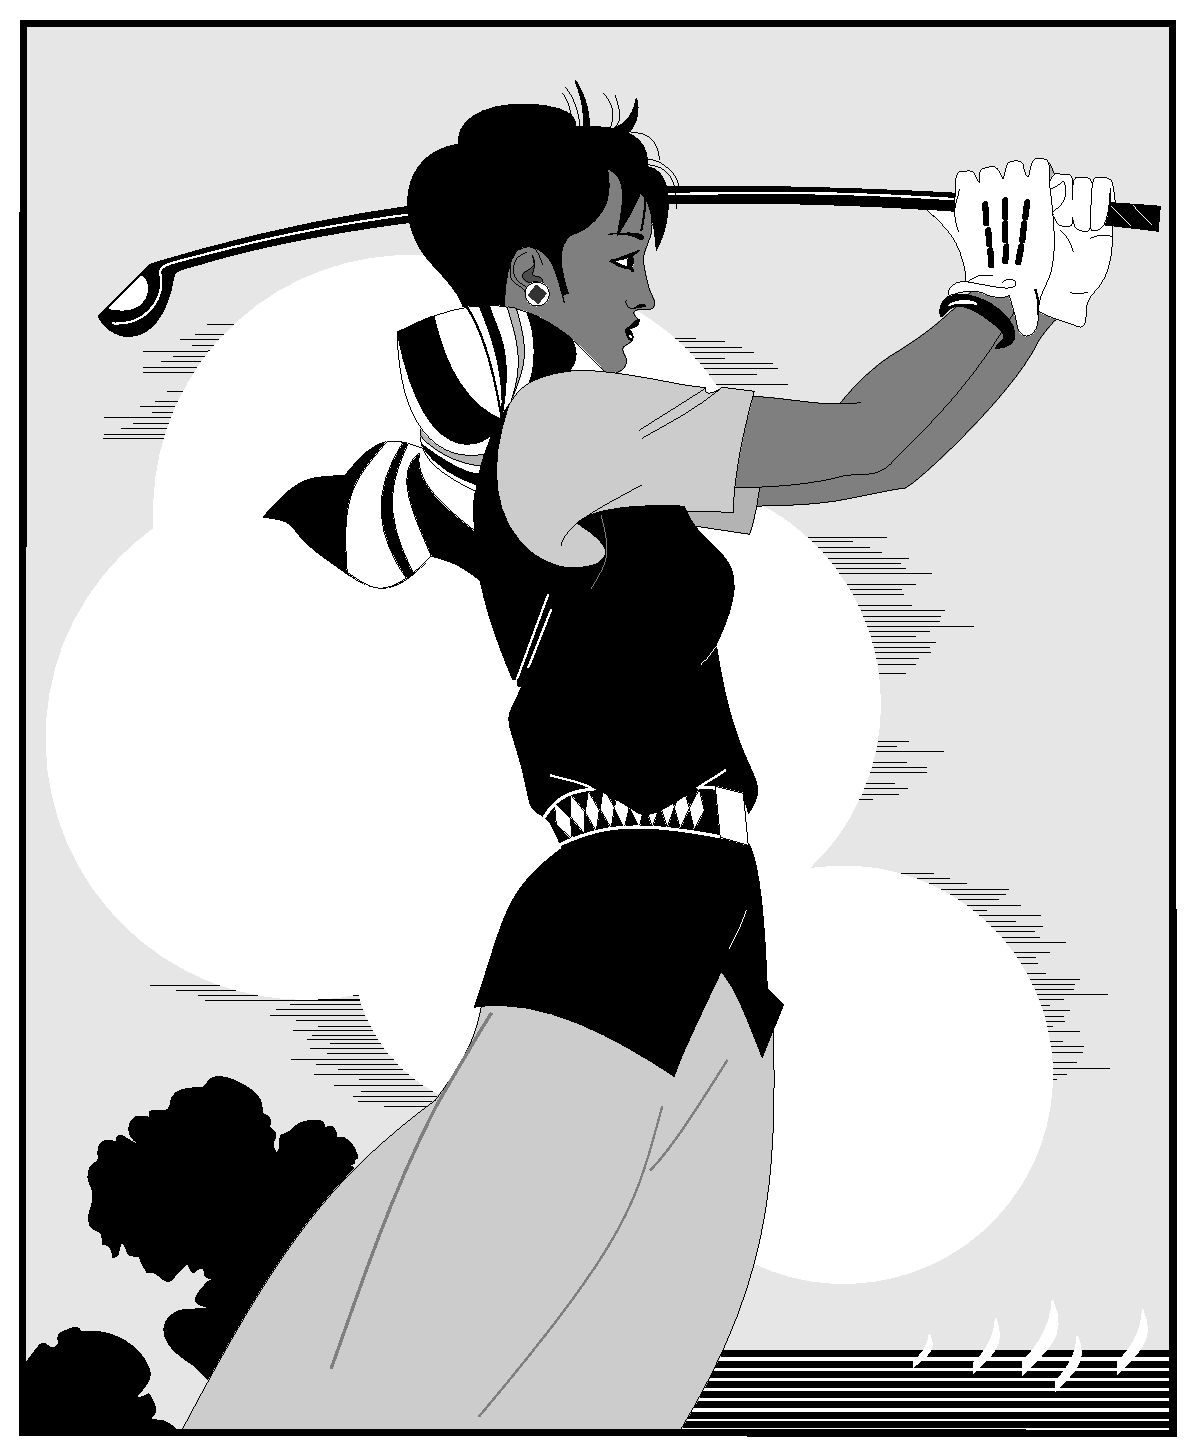
\includegraphics[width=0.2\textwidth]{golfer}}
\bicaption[golfer7]{}{打高尔夫球的人(非规范要求)}{Fig.$\!$}{The person playing golf (Not stated in the regulation)}
		\end{minipage}
	\end{sideways}
\end{figure}

\clearpage

如果不想让图片浮动到下一章节,那么在此处使用\cs{clearpage}命令。

\section{如何做出符合规范的漂亮的图}

关于作图工具在后文\ref{drawtool}中给出一些作图工具的介绍,此处不多言。
此处以R语言和Tikz为例说明如何做出符合规范的图。

\subsection{Tikz作图}

使用Tikz作图核心思想是把格式、主题、样式与内容分离,定义在全局中。
注意字体设置可以有两种选择,如果字少,用五号字,字多用小五。
使用Tikz作图不会出现字体问题,字体会自动与正文一致。

\subsection{R作图}

R是一种极具有代表性的典型的作图工具,应用广泛。
与Tikz图不同,R作图分两种情况:(1)可以转换为Tikz码;(2)不可转换为Tikz码。
第一种情况图形简单,图形中不含有很多数据点,使用R语言中的Tikz包即可。
第二种情况是图形复杂,含有海量数据点,这时候不要转成Tikz矢量图,这会使得论文体积巨大。
推荐使用pdf或png非矢量图形。
使用非矢量图形时要注意选择好字号(五号或小五),和字体(宋体、新罗马)然后选择生成图形大小,注意此时在正文中使用\cs{includegraphics}命令导入时,不要像导入矢量图那样控制图形大小,使用图形的原本的
宽度和高度,这样就确保了非矢量图形中的文字与正文一致了。

为了控制\hitszthesis\ 的大小,此处不给出具体举例。

\subsection{专业绘图工具}[Processional drawing tool]
\label{drawtool}

推荐使用tikz包,使用tikz源码绘图的好处是,图片中的字体与正文中的字体一致。具体如
何使用tikz绘图不属于模板范畴。

tikz适合用来画不需要大量实验数据支撑示意图。但R语言等专业绘图工具具有画出各种、
专业、复杂的数据图。R语言中有tikz包,能自动生成tikz码,这样tikz几乎无所不能。
对于排版有极致追求的小伙伴,可以参考
\href{http://www.texample.net/tikz/resources/}{http://www.texample.net/tikz/resources/}
中所列工具,几乎所有作图软件所作的图形都可转成tikz,然后可以自由的在tikz中修改
图中内容,定义字体等等。实现前文窝工规范中要求的图中字体的一致性的终极目标。

\lipsum[1]

\section{本章小结}[Brief summary]

\lipsum[1]
